% Modes
%  draft - drafting mode, esp for todos
%  final - final mode
%
% Other
%  print - do not color links
%

\PassOptionsToPackage{final}{graphics}

\documentclass[draft,master]{swathesis}

% my additions --- begin

\KOMAoptions{parskip=true}

\lstset{language=JavaScript,extendedchars=true}

\usepackage{pifont}
\newcounter{dingdistance}
\setcounter{dingdistance}{191}
\newcommand{\circnum}[1]{%
  \addtocounter{dingdistance}{#1}%
  \ding{\value{dingdistance}}%
  \setcounter{dingdistance}{191}}

\addbibresource{thesis.bib}

% my additions --- end


\usepackage{titlepage}
\TitlePageStyle[
subject=master,degree={Master of Science},
]{hpi-swa}

\supervisors{
Prof.\,Dr.\,Robert Hirschfeld\and
Bastian Steinert
}

% ABGABEDATUM
% \setdate{2012}{04}{05}
% \date{\datedate}

\author{Lauritz Thamsen}
\location{Potsdam}
\extratitle{\raggedleft Thamsen, \\ Object Versioning for the Lively Kernel\par}
\title{Object Versioning for the Lively Kernel}
\subtitle{Preserving Access to Previous System States\\ in an Object-oriented Programming System}

\begin{document}
\frontmatter
\maketitle
%
% abstract.tex
% Abstract / Zusammenfassung
%
\begin{abstract}

% Background
In programming systems such as the Lively Kernel programmers construct applications from objects.
Dedicated tools allow them to manipulate the state and behavior of objects at runtime.
Programmers are encouraged to make changes directly and receive immediate feedback on their actions.

% Problem Statement
When programmers, however, make mistakes in such programming systems, they need to undo the effects of their actions.
Programmers either have to edit objects manually or re-load parts of their applications.
Moreover, changes can spread across many objects.
As a result, recovering previous states is often error-prone and time-consuming.

% Approach
This thesis introduces an approach to object versioning for systems like the Lively Kernel.
Access to previous versions of objects is preserved using \emph{version-aware references}.
These references can be resolved to multiple versions of objects and, thereby, allow re-establishing preserved states of the system.

% Results
We present a design based on proxies and an implementation in JavaScript.
An evaluation shows that the Lively Kernel can run with our proxy-based version-aware references and that preserved system states can be re-established.
The memory overhead of the version-aware references is reasonable.
The execution overhead is not yet practical.
% Conclusion
However, with performance improvements, the solution could be used to provide practical recovery support to programmers.

\end{abstract}




\begin{zusammenfassung}

In Programmiersystemen wie dem Lively Kernel können Programmierer Anwendungen aus Objekten erstellen.
Dabei erlauben dedizierte Werkzeuge den Zustand und das Verhalten von Objekten zur Laufzeit zu verändern.
Programmierer werden ermutigt Änderungen direkt zu machen und erhalten umgehend Feedback.

Wenn Programmierer in solchen Programmiersystemen aber Fehler machen, müssen sie Änderungen rückgängig machen.
Dazu müssen sie entweder Objekte manuell bearbeiten oder Teile ihrer Anwendungen neu laden.
Die gemachten Änderungen können dabei über viele Objekte verteilt sein.
Vorherige Zustände wiederherzustellen ist deshalb häufig schwierig und zeitaufwendig.

Diese Arbeit stellt einen Ansatz für die Versionierung von Objekten in Systemen wie dem Lively Kernel vor.
Der Ansatz basiert auf \emph{Versions-bewussten-Referenzen}.
Diese können zu mehreren Versionen von Objekten aufgelöst werden und erlauben so vorherige Systemzustände wiederherzustellen.

Für den Ansatz beschreibt diese Arbeit eine auf Proxys basierenden Implementierung in JavaScript.
Eine Evaluierung davon zeigt, dass die Implementierung es erlaubt Systemzustände des Lively Kernels zu erhalten und wiederherzustellen.
Der zusätzlich nötige Arbeitsspeicher für die Versions-bewussten-Referenzen ist dabei vertretbar, während die Programmausführung erheblich verlangsamt wird.\\
Mit Verbesserungen könnte die Lösung allerdings benutzt werden, um Entwickler mit praktikablen Wiederherstellungs-Werkzeugen zu unterstützen.

\end{zusammenfassung}

%%% Local Variables:
%%% mode: latex
%%% End:

\begingroup
\let\raggedsection\centering

\chapter*{Acknowledgments} \label{cha:acknowledgments}
\endgroup

\begin{quotation}
  \noindent I am grateful to my supervisors Bastian Steinert and Professor Robert Hirschfeld for their guidance and support. 
\end{quotation}

\begin{quotation}
  \noindent I am thankful to Jens Lincke, Marcel Taeumel, Tobias Pape, Tim Felgentreff, Michael Perscheid, Stephanie Platz, Carl Friedrich Bolz, Robert Krahn, and Dan Ingalls for fruitful discussions and valuable input.
\end{quotation}

\begin{quotation}
  \noindent I thank Oliver Buck for his comments on drafts of this thesis.
\end{quotation}
\tableofcontents
\listoffigures
% \listoftables
% \lstlistoflistings
% \listofacronyms
\mainmatter

% I. Background and context (problem area and motivation) 
% II. However (problem description)
% III. So what? (problem dimension) 
% IV. Deficiencies with previous approaches
% IV. Solution

\chapter{Introduction} \label{chapter:INTRODUCTION}

% Background
Programming systems such as Squeak/Smalltalk~\cite{Ingalls1997Squeak,GoldbergRobson83} and REPLs for LISP or Python allow to adapt and develop programs while those run.
Changes to programs in such environments are effective immediately and programmers can often see or test right away what differences their actions make.
Thus, these systems provide immediate feedback to programmers.
A subset of such systems, which includes, for example, Self~\cite{Ungar1987SPS,Ungar2007SEL} and the Lively Kernel~\cite{Ingalls2008LKS,Krahn2009LWD}, are those built around prototype-based object-oriented languages, in which programmers create applications using objects and without having to define classes first.
In these systems, programmers can inspect and change the state of objects at runtime and can add and modify object-specific behavior.
The results of such development are actual objects, not source code that only abstractly describes potential objects.

The Lively Kernel was designed to support this kind of development and focuses, hereby, on graphical objects.
For this, the Lively Kernel provides tools to directly manipulate the style, the composition, and the scripts of graphical objects.
For example, programmers can change positions and the composition directly using the mouse.
They can edit and try methods directly in the context of graphical objects, or use temporary workspaces to manipulate one or many objects programmatically.
For example, to add new functionality to a graphical application, a programmer might copy an existing button object and then directly modify the newly button object: move the new button to a sensible position, resize it slightly, set a new label, and add a script to be executed on each mouse click.
The programmer makes all these changes directly to one button object and, for example, how the button fits into the application's interface is visible at all time, while clicking the button allows to directly test its functionality.
This way, the Lively Kernel often allows for fast feedback, especially during the development of graphical applications.

% Problem
Changes programmers make to objects---either using specific tools or through executing code---can, however, also turn out not to be improvements and still permanently affect objects.
Programmers can, for example, accidentally change the positions, accidentally connect the wrong objects when manipulating applications with mouse interactions, or make a mistake in a workspace code snippet that then manipulates many objects differently than intented.
Similarly, programmers might learn in hindsight that making a promising change to an object's scripts actually introduced an error or impacts the application's performance.
Less accidental but still problematic, they might try a couple of different alternatives as, for example, different color schemes and graphical layouts, only to realize later that an earlier state was most appealing and should thus be re-established.
Other potentially inappropriate changes might be introduced when code is evaluated to understand or test behavior, not to permanently change state.

% So what?
When changes, however, do turn out to be innapropriate, programmers often need to undo them manually or need to have prepared for potential negative outcomes in advance.
That is, the Lively Kernel does not provide an undo for changes to objects, which is especially at odds with the Lively Kernel's support for trying ideas right away: Developers are able to make changes directly and frequently receive immediate feedback, but do not get support when changes turn out to be inappropriate.
So, when programmers want to recover a previous development state, they often need to manually reset the state to how it previously was---often using the same tools the changes were initially made with and potentially involving multiple properties of multiple objects changed by multiple developer actions.

The Lively Kernel provides tools to commit and load versions of objects.
In case such commits exist, programmers can load earlier versions of objects to re-establish previous states.
Nevertheless, depending on how far such a commited version is from the actually desired state, manual changes might still be necessary.
Thus, to keep the effort required to re-establish \emph{any} previous state low, programmers would need to commit many versions.
However, these commits would partly be made only to preserve intermediate development states, not to share and document work results but to protect against changes that unexpectedly turn out to be mistakes.
The commits would further also require significant effort, especially when the preserved versions should be usable and documented, requiring states to be either tested and augmented with useful descriptions right away, or else requiring developers to actively clean up repository histories regularly.\\
\emph{In summary}, recovering previous states of objects in the Lively Kernel is currently a significant effort for programmers as they either have to manually re-set changed state or to take significant precautionary actions.\\

A typical approach to implementing multi-level undo for the changes to state of applications is the Command pattern~\cite{GammaHelmJohnsonVlissides95}.
The command pattern packages changes into actions.
It can then record actions and, when each action has been provided with an undo counterpart, subsequentely undo them.
This, however, requires developers to implement specific undos for all possible actions, which even for just the existing tools to manipulate objects in the Lively Kernel would result in a rather comprehensive implementation and which would of course also require developers to accompany each newly implemented manipulation tool with undos.  
Further, this approach is entirely unpractical for undoing the effects of evaluating arbitrary code snippets as, for example, regularly done in the Lively Kernel's workspaces.

Worlds~\cite{Warth2011Wor} is a recent and more generic approach using a language construct for controlling the scope of side-effects from arbitrary code.
It allows to capture the side-effects of statements into different \emph{worlds}.
These worlds can be used to run code with particular sets of changes being effective.
Developers could, thus, execute all their actions in separate worlds and discard those worlds when necessary to return to previous ones.
Worlds as such, though, would require developers to explicitly create as well as potentially merge or discard worlds, and, therefore, still needs the programmer to explicitly take precautionary actions, similar to version control systems.
In addition, the implementation of Worlds for and in JavaScript is not yet practical as it, for example, currently prevents garbage collection.

In contrast to these approaches, CoExist~\cite{Steinert2012COE,Steinert2014EVA} provides automatic recovery support, without requiring developers to take any precautionary actions beforehand.
For this, CoExist automatically records versions for every change and, thereby, provides a fine-grained history of intermediate development states.
To each preserved version programmers can also see diff views, screenshots, and test results.
Programmers can review the changes chronological, examine the impact each change had, and re-establish previous development states again.
However, CoExist currently recognizes only changes made to the source code of classes and does not preserve the state of objects.

% Solution
This thesis proposes to version the entire state of programming runtimes as basis for automatic recovery support in systems like the Lively Kernel.
In particular, this thesis introduces an approach to preserving and managing versions of all objects, which make up different runtime states, using alternative, \emph{version-aware} references.
Version-aware references are alternative references in that they can refer to multiple versions of objects, but always resolve transparently to one particular version among those.
Versions of objects are preserved together, so that the version-aware references can be resolved transitively to state as it was at a particular moment.
For this to be practical, versions of objects can be kept in application memory and the state of all objects can be preserved incrementally, on writes and only for objects that actually change.
Similarly, to which versions the version-aware references resolve can also be changed without significantly interrupting program execution:
The version-aware references can decide dynamically to which versions they resolve instead of being hard-wired to specific versions.

We implemented version-aware references for the Lively Kernel in JavaScript, on the level of the language using proxies and source transformations and, thus, without requiring adaptions to established execution engines.
Proxies implement version-aware references.
They stand in for references: conventional references point to them and they delegate all object access--all kinds of read and write operations--transparently to one particular version of the object they can stand in for.
A combination of proxy behavior and source transformation then allows to introduce and use these proxies consistently for all objects, in order to version the entire runtime state as is necessary for completely generic recovery support.

We designed and implemented this approach to object versioning for the Lively Kernel with the intention to provide CoExist-like recovery support, including continuous versioning, in the future.
Therefore, this approach supports fine-grained histories of development states---many, but still particular versions of the entire runtime that can correspond to developer actions and can be re-established quickly.
It also allows to easily enhance preserved development states with further information as, for example, test results, screenshots, and diffs.
That is, in the future, we want to build upon the presented solution and support developers in efficiently recovering state from continuously preserved, fine-grained histories of development sessions.

\section{Contributions}

The goal of this work is to provide a basis for automatic recovery support for systems like the Lively Kernel.
To that effect, the main contributions of this thesis are the following:

\begin{itemize}
    \item An approach to object versioning for systems like the Lively Kernel based on alternative, version-aware references that transparently delegate to one of multiple versions of an object (Section~\ref{sec:APPROACH:1}).
    \item A concrete, language-level solution that provides the proposed version-aware references through proxies and source transformations for the Lively Kernel (Section~\ref{sec:APPROACH:2}).
    \item An implementation of the concrete solution in JavaScript that can be used to effectively preserve and re-establish development states of the Lively Kernel (Section~\ref{chapter:IMPLEMENTATION}).
\end{itemize}


\section{Thesis Structure}

The remainder of this thesis is organized as follows. 
Chapter~\ref{chapter:BACKGROUND} describes prototype-based programming systems, CoExist, and the Lively Kernel.
Chapter~\ref{chapter:MOTIVATION} illustrates how developers directly manipulate objects in the Lively Kernel and exemplifies characteristic recovery needs associated with this kind of development.
Chapter~\ref{chapter:APPROACH} introduces our approach to object versioning and describes how proxies can be used for concrete solutions.
Chapter~\ref{chapter:IMPLEMENTATION} presents our implementation for the Lively Kernel, which Chapter~\ref{chapter:EVALUATION} then evaluates in terms of functionality and practicability.
Chapter~\ref{chapter:RELATED_WORK} compares our solution to related work.
Chapter~\ref{chapter:FUTURE_WORK} presents future work, while Chapter~\ref{chapter:CONCLUSION} concludes this thesis.

\chapter{Background} \label{chapter:BACKGROUND}

Our goal is to provide generic recovery support for prototype-based programming systems and we implemented our approach for the Lively Kernel, a particular example of such a system.
Prototype-based programming systems use objects directly as building blocks for applications without requiring more abstract entities like classes.
The Lively Kernel is a prototype-based, self-supporting, and web-based programming system with tools to directly manipulate graphical objects.

Our approach and the implementation are intented to provide similar automatic recovery support to programmers as CoExist does.
CoExist applies continuous versioning to provide programmers with access to a fine-grained history of development states without requiring them to take any explicit precautionary actions themselves.


\section{Prototype-based Programming}

Prototype-based programming is object-oriented programming in which applications are constructed using only objects, without classes.
Examples for programming languages or systems that implement prototype-based programming are Self, JavaScript, and Kevo~\cite{Taivalsaari1992Kevo}.
Self and JavaScript incorporate prototypical inheritance.
They allow objects to inherit state and behavior directly from other objects: an object has a prototype to which it delegates when looking up a property in the object itself yields no results.
Kevo, in constrast, does not provide this kind of delegation, but instead allows to make full copies of objects, so objects in Kevo do not share behavior or state.
Programmers can create new objects with initially the same state and behavior as existing ones, but all objects remain self-contained.
That is, in Kevo, changing an object only changes that particular object and a particular object can only be changed by directly changing it, not by changing any other artifact.
To adapt many objects at once Kevo, programmers can only use so-called \emph{module operations} that are evaluated on a group of objects. 
Despite this difference in whether properties can be shared among objects and how to then affect families of objects, prototype-based programming always allows to build programs from particular objects, in contrast to the class-based style of object-oriented programming, in which programs are defined in abstract descriptions of structure and behavior.
In particular, the parts of a program are objects with particular state, specific examples rather than general categories.

There are different advantages associated with this kind of programming:
\begin{itemize}
    \item \cite{Taivalsaari1996CVP} and \cite{Ungar1987SPS} argue that it might be easier for programmers to understand concrete examples compared to abstract classes. A concrete example provides particular values for its state and, in case of objects with a visual appearance, can be actually looked at.
    \item \cite{Ungar1987SPS} and \cite{Borning1986CVP} describe how prototype-based programming makes it easier to introduce one-of-a-kind objects with their own structure or behavior.
    \item \cite{Borning1986CVP} and \cite{Maloney1995Mor} make the point that especially editing visual objects can be more concrete with prototypes. Instead of writing code to define the appearance of objects, programmers can manipulate particular visual objects directly. Programmers could, for example, use the mouse to manipulate properties like the size, position, and style or to combine multiple basic elements into one composition. This way, programmers always see intermediate states and do not only receive feedback on explicit test runs in-between edit-compile-load cycles or run/edit distinctions. 
\end{itemize}

Similarly to the previous examples, many end-user programming systems, including Scratch\cite{Maloney2010SPL}, Etoys~\cite{Kay2005Etoys}, and Fabrik~\cite{Ingalls1988FVP}, enable users to express their programs through particular objects, all with graphical representations and tools to directly manipulate those.
In addition, programmers manipulate objects at runtime both in these end-user programming systems and in many general-purpose prototype-based programming systems like the Lively Kernel, Self, and Kevo.
Further, most of these systems also provide tools for manipulating graphical objects directly, where graphical objects range from simple objects like primitive shapes over interactive widgets to applications like presentation software or programming tools.
In general, programming at runtime, prototype-based programming, and direct manipulation of graphical objects seem properties that suit each.


\section{The Lively Kernel}

The Lively Kernel is a browser-based programming system in the tradition of both Smalltalk and Self.
Development in the Lively Kernel happens at runtime and it incorporates tools and techniques to be completely self-sufficient.
Thus, pogrammers can create versions of the Lively Kernel with the Lively Kernel.

The Lively Kernel is based in the JavaScript programming language.
Therefore, the system and applications are expressed in a prototype-based object-oriented language that also provides prototypical inheritance.
At the same time, the Lively Kernel also provides a class system for JavaScript and considerable parts of the system itself are expressed using this class system.
One of these parts expressed through classes is an implementation of Morphic~\cite{Maloney1995Mor}, a framework for developing graphical applications.
Programmers can alter graphical objects of this framework, which are called \emph{Morphs}, using direct manipulation and through a number of dedicated tools.
While the framework and other parts of the core system are expressed using classes, these morphs are an example of objects that are often edited directly and not through adapting existing or creating new classes.
Though each morph does have a class, it can have not only its own state, but object-specific behavior---thus the Lively Kernel effectively mixes the prototype-based and the class-based flavors of object-oriented programming.

\begin{figure}[h]
    \centering
    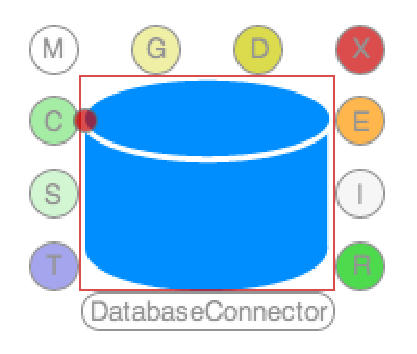
\includegraphics[width=0.3\textwidth]{figures/2_background/1_halos.pdf}
    \caption{The halo buttons of a simple morph.}
    \label{fig:Halos}
\end{figure}

Programmers can change the position of morphs by dragging and the composition by an alternative dragging, which is called \emph{grabbing}.
That is, the composition of morphs is also part of Morphic and a morph can have submorphs.
This way, morphs are not limited to to be basic shapes or simple widgets, but can be entire user interfaces of arbitrary applications.
The Lively Kernel provides a set of manipulation tools, called \emph{Halos}, as shown in Figure~\ref{fig:Halos}, that developers can bring up directly at morphs.
The different halo buttons allow, for example, to resize~\textcircled{R}, rotate~\textcircled{T}, and copy~\textcircled{C} morphs.
The copy operation does not establish a prototypical inheritance relationship between the copy and the original, but instead copies the entire state, including of which class the copy is an instance.
Other halo buttons open specific tools, which are shown in Figure~\ref{fig:LivelyTools} to further manipulate the morphs:

\begin{enumerate}
    \item The \emph{Inspector}~\textcircled{1} presents all the values that make up a morph's state. It also has a small code pane at the bottom, which is intended to be used to manipulate the state programmatically.
    \item The \emph{Style Editor}~\textcircled{2} allows to manipulate certain aspects of a morph's visual appearance. Programmers can use it to, for example, change a morphs color, border width, or the layout of its submorphs.
    \item The \emph{Object Editor}~\textcircled{3} is a tool dedicated to the object-specific behavior of morphs, which are called \emph{scripts} in the Lively Kernel. It shows all scripts of a particular morph, but also can add and adapt scripts.
\end{enumerate}

\todo{smaller numbers in the Figure..}

\begin{figure}[h]
    \centering
    \includegraphics[width=\textwidth]{figures/2_background/2_LivelyTools.pdf}
    \caption{The Lively Kernel's tools to manipulate properties of morphs, from left to right: the Inspector, the Style Editor, and the Object Editor.}
    \label{fig:LivelyTools}
\end{figure}

\begin{figure}[h]
    \centering
    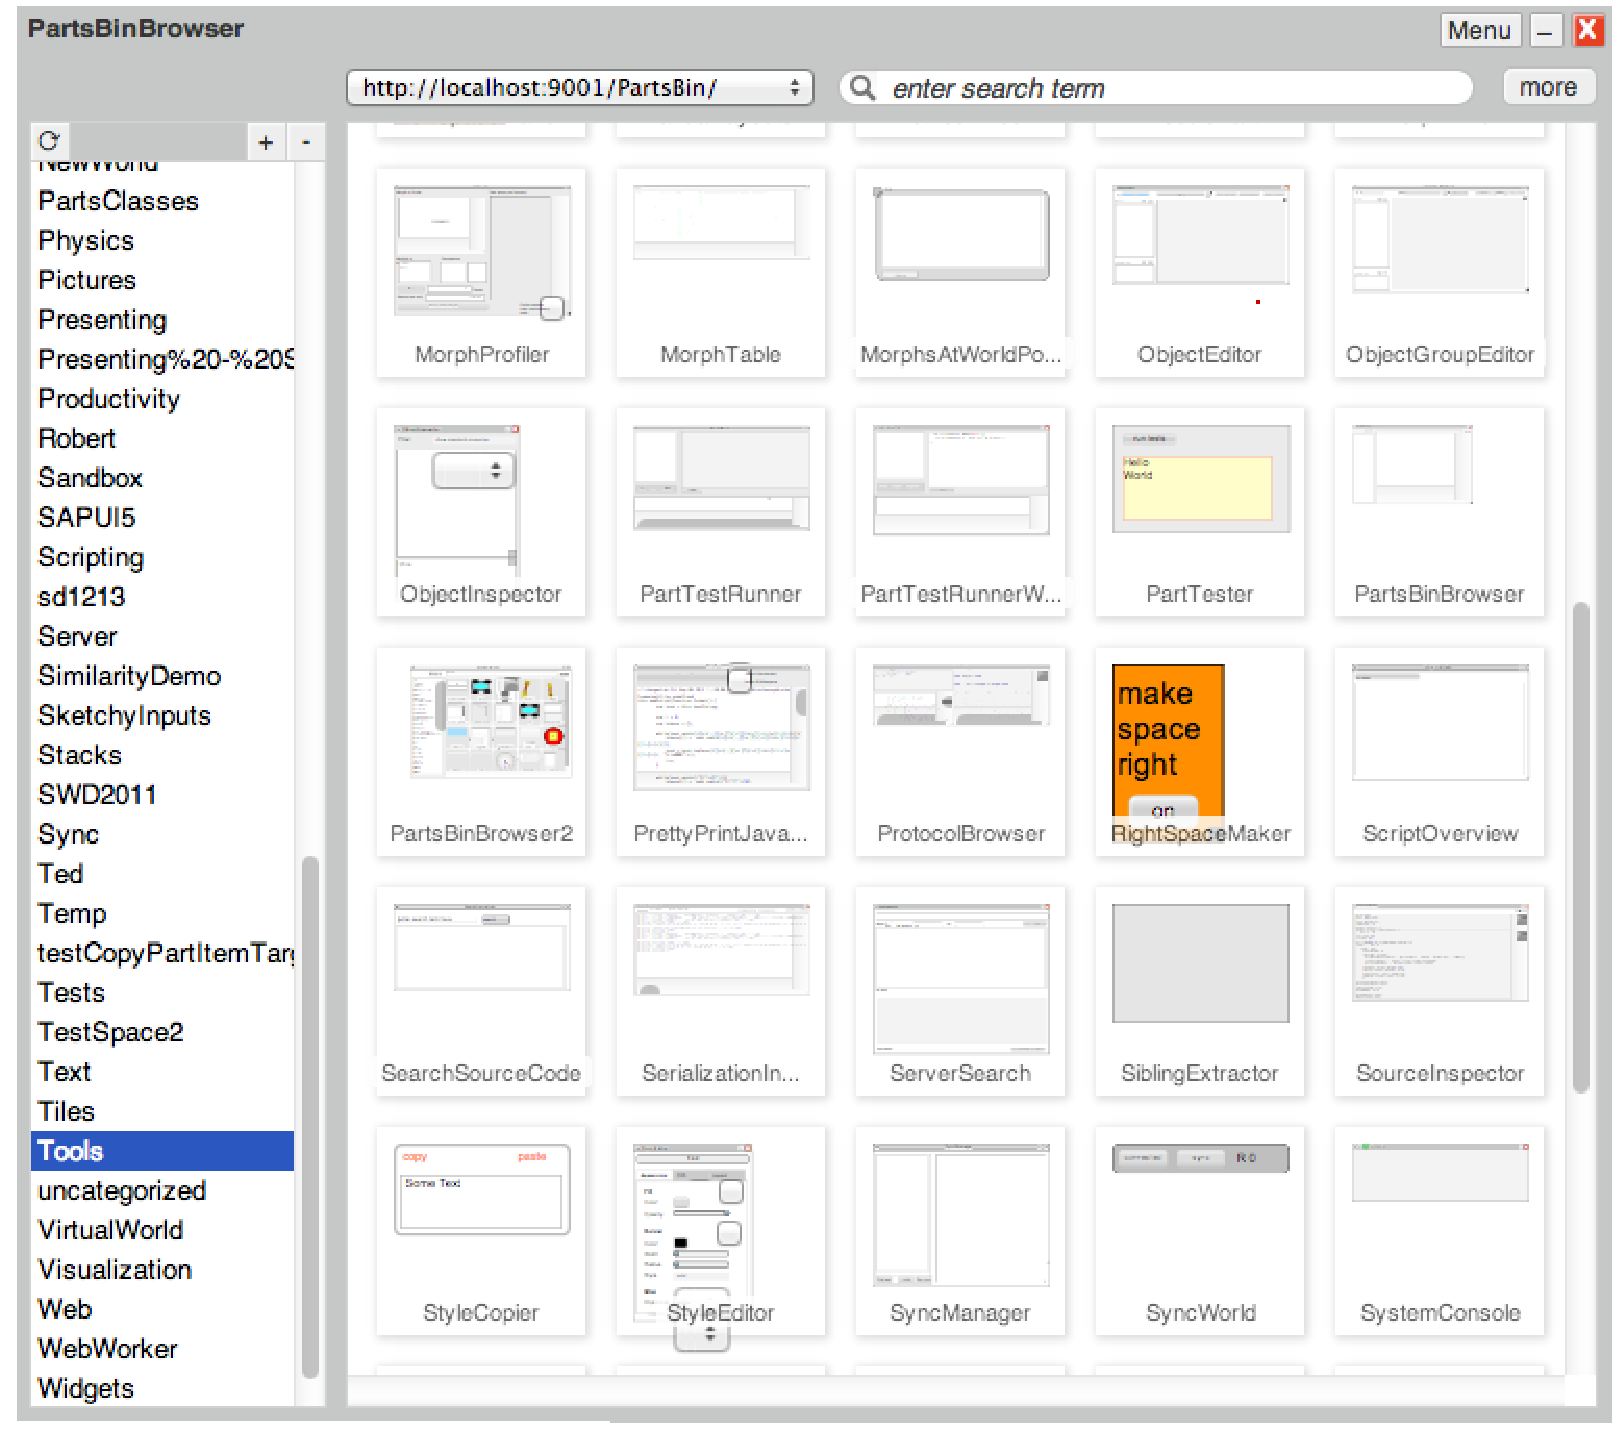
\includegraphics[width=0.7\textwidth]{figures/2_background/3_partsBin.pdf}
    \caption{The Lively Kernel's Parts Bin opened on the \emph{Tools} category.}
    \label{fig:PartsBin}
\end{figure}

Another tool related to morphs, though not available from a halo button, is the Lively Kernel's \emph{Parts Bin}~\cite{Lincke2012LPC}, an object repository to commit and load specific versions of morphs.
Morphs saved to the Parts Bin are called \emph{parts} to emphasize the ability to reuse any one of the morphic applications stored in the Parts Bin for other applications.
Figure~\ref{fig:PartsBin} shows the Parts Bin and, in particular, a group of tools that the Parts Bin contains, which includes both the Style Editor and the Object Editor.
Both these tools are examples for graphical applications developed from available parts, with their logic expressed in scripts, and available to users through the Parts Bin.


\section{CoExist}

The CoExist system\footnote{\url{http://www.bastiansteinert.org/coexist.html}, accessed February 28, 2014} and approach supports programmers through automatic and continuous versioning.
CoExist preserves each indermediate development state with its respective source code and associated runtime information.
The states are recorded as separate version in their original order and along with change summaries, associated test results, and screenshots of the development environment.
Programmers can review their development sessions, inspect the impact each individual change had on test cases, and recover previous development states.
They can completely withdraw withdraw changes or only re-visit a previous state to recover partial information as, for example, the source code for a specific method.

\begin{figure}[h]
    \centering
    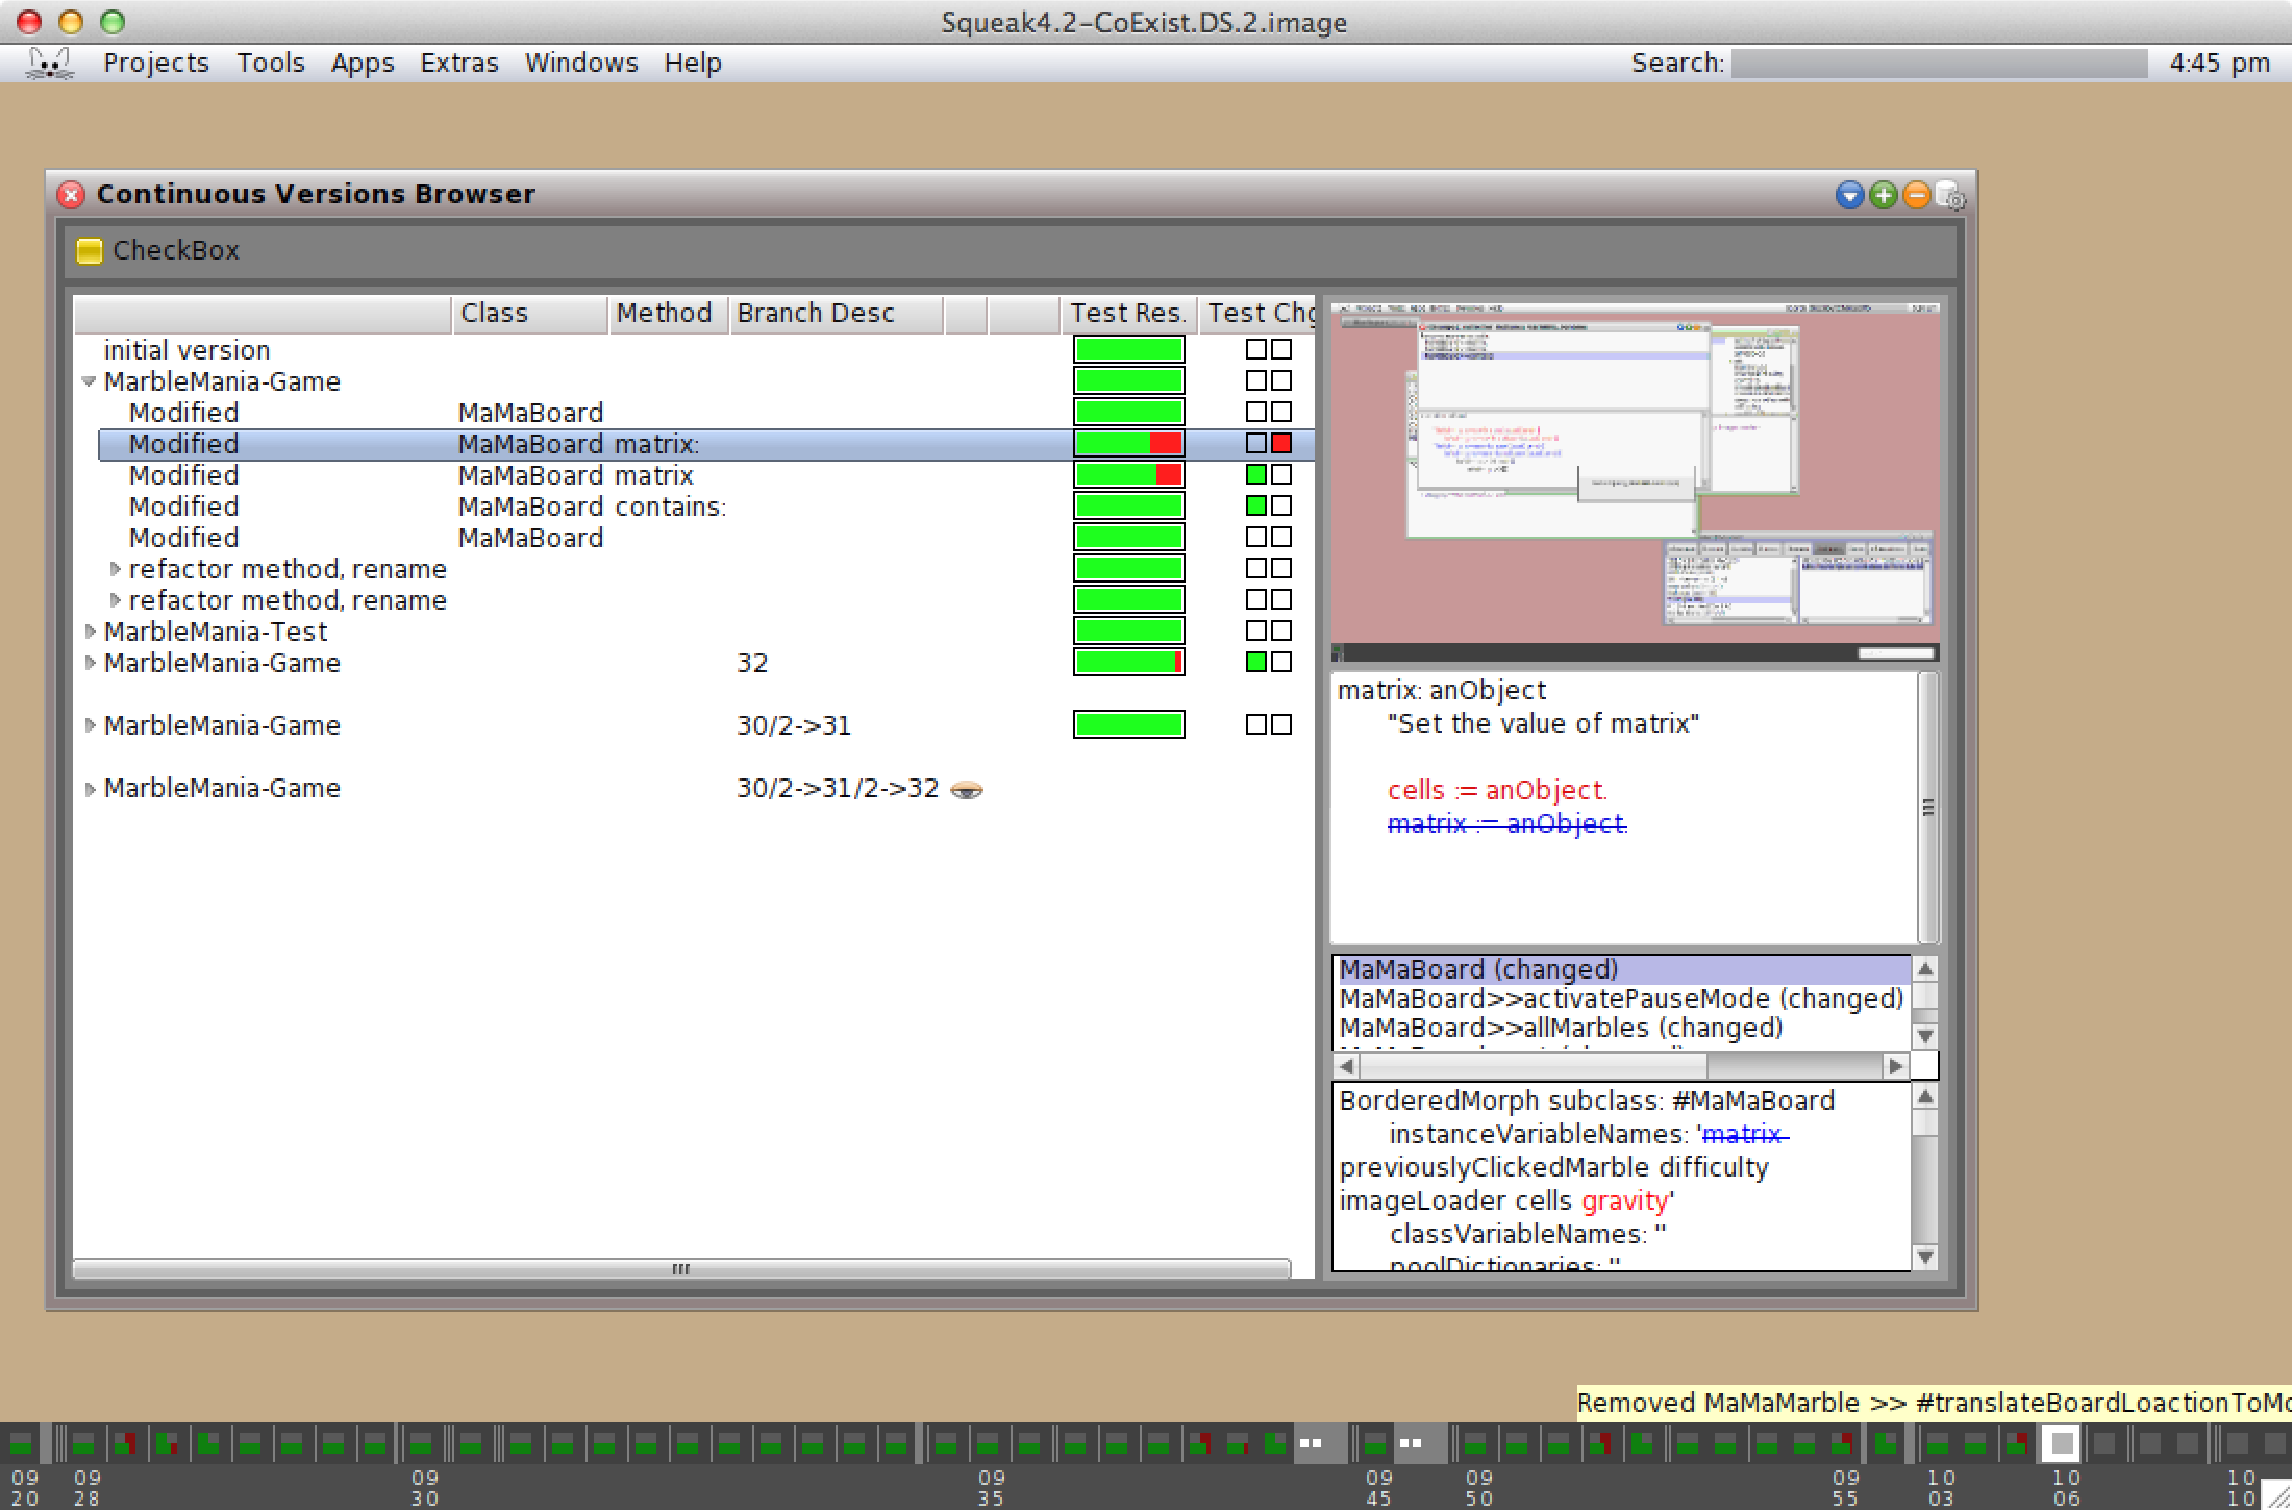
\includegraphics[width=\textwidth]{figures/2_background/4_coexistTools.pdf}
    \caption{CoExist's tools to manage the preserved development states: a timeline and a Version Browser.}
    \label{fig:CoExist}
\end{figure}

CoExist provides tools to help programmers benefit from the preserved development histories, shown in Figure~\ref{fig:CoExist}.
A timeline tool at the bottom of the development environment presents each intermediate version through a small rectangle that indicates the impact on test cases: the bottom of the rectangle shows how many test cases passed and failed absolutely, while the top half highlights only test results affected by the changes of this particular version.
Hovering above such a version rectangle indicates what exactly changed in terms of methods and classes.
Clicking a version provides access to its source code and more information on test results, but also allows to re-establish the version.
Besides this timeline of versions, a Version Browser tool shows changes in a different structure, also chronological, but separately for different source code modules.
It presents the same information on test cases, but in addition also offers diffs and how the development environment appeared visually in each version through providing screenshots.
The two tools support programmers in re-tracing their steps, understanding the impact of their actions, and in recovering information from previous development states.

CoExist is intented to reduce the effort that programmers usually put into recovery, either into actual compensational actions or into precautionary actions, and, thereby, also to help programmers to overcome any aversions to try new ideas.
To re-establish a previous development state---because of, for example, unintentionally introduced errors, decreased performance, or harmed program design---programmers can manually repair improperly changed code or load a previously commited version of the sources.
Programmers can preserve specific versions to be able to easily withdraw changes, and, thereby, reduce the cost of recovery by anticipating recovery needs beforehand.
However, preserving versions manually is also an effort and especially so when revision histories are expected to be well-documented and immediately useful.
For that, programmers need to assemble changes to meaningful increments, test these, and write helpful commit messages.
Testing each one directly is also advocated as it can help to find introduced problems directly intead of later analyzing long lists of changes that all could potentially have introduced a problem.
With CoExist, developers do not have to take these explicit precautionary actions, but still have access to a fine-grained history of development states and even test results for each individual state.
Instead of worrying about negative consequences when trying ideas, programmers can focus on their actual programming tasks and rely on CoExist to help in case any action unexpectedly needs to be undone.

% \todo{Structured: not just like auto-save (google docs), but structured: associated with particular actions and the static structure of programs... class>>method (add/delete/modify).. and also cross-document}

% % sometimes easier to make the changes and experience the results than to anticipate the changes beforehand...)

% have to remember to make commits +  
% commits take some effort: combining changes into meaningful increments, making sure the current version passes test cases, where test cases also take time, writing helpful commit messages
% for this reason, not a commit for every single change, but deciding when to commit, assessing the risks of changes and planning changes to a point where grouping changes into consistent steps, which each should be commited separately, is also time-consuming and error-prone

\chapter{Motivation} \label{chapter:MOTIVATION}

In Lively, programmers can create applications by manipulating and composing simpler parts.
These graphical objects can be edited using a variety of direct manipulation tools.
When programmers do edit these parts directly, they often see the effects of their actions immediately.
However, not all these effects are improvements and sometimes programmers want to undo recent changes and recover previous situations.
The development of parts in Lively and conceivable recovery needs are shown by the example of adding a new functionality to an existing tool in Lively.


\section{Part Development In Lively}

To exemplify how developers change objects directly in Lively, we will add a new feature to Lively's Object Editor.
The editor itself has been been developed by composing and editing simple graphical objects like buttons, text fields, and lists.
For this reason, we do not have to adapt any source code modules to change the editor, but rather manipulate and save the concrete editor object.
The new feature we add in this example is a magnifier button that can show the editor's current target.
The target is the object to which the Object Editor currently presents scripts to and allows to manipulate.
This requires to create and add a new button morph to the editor, as shown in Figure TODO.
Subsequentely, the magnifier button also needs some behavior.
The magnifier feature helps to accomplish two specific tasks: First, when a programmer hovers over the button, the Object Editor's current target object is highlighted through a blue and transparent overlay. Second, when a programmer clicks the button, the current target selection is revoked and the programmer can visually select the new target of the editor.
This example covers the first of these two behaviors, which is also visible in Figure TODO.

\todo{add a before-and-after-screenshots figure and one figure that shows how the magnifier works ()}


\todo{add a bit more details in to the following text and a Figure that shows the various steps of this example,.. refer to the steps in the text.. also add more details to how the scripts work..}

The first step is copying an existing button object or loading a button object from Lively's Parts Bin.
We then can use the button's halos, in particular the resize tool, to give the button a smaller and square extent.
Next, we can load an image showing a magnifier.
Using drag and drop we can add the image to the button and the button to the editor.
Dropping a morph onto another structurely connects morphs in Lively.
That is, moving the editor around will also move the button with its image accordingly, while saving will respectively include both the button and the image.
Besides manipulating the state of the button, image, and editor objects---using mouse interactions to set their extents, their positions, and connect them---we would probably next add some object-specific behavior.
First, we can add scripts to the button that while the mouse cursor hovers above it, a translucent rectangle is layed over the current target, highlighting the morph that is currently being edited.



\section{Recovery Needs When Developing Parts}

\todo{this whole section needs to be more concrete and actually present situations from the previously introduced example. e.g. explain how parts of the script to can be evaluated to test whether the overlay works, but even when that works as intented there is then just wrong state (an overlay added to some morph in the world..)}

While manipulating objects directly, developers might make changes to object state that they subsequentely want to undo.
In the previously summarized example developers might, for example, developers might accidentally move the new button after carefully positioning it.
Or they might accidentally drop the button into an existing layout, thereby undesirably repositioning multiple unrelated morphs.
An extreme example for such an accidental inappropriate change is closing a morph that had meaningful, but unsaved changes.

In constrast to those clearly undesired, accidental changes, well-intentioned changes can also result in the desire to recover a previous development state.
For example, when fine-tuning the visual appearance of a morph, a developer might make many changes to the sizes, the positions, and the colors of morphs, only to decide later-on that a particular intermediate version was most appealing.
Or developers edit a script only to learn that the change introduced an an error or a decrease in performance.
Further, developers can change objects not only through direct manipulation, but also could write a code snippet that makes changes to the state or behavior of an objects.
Such a snippet could of course change any number of properties of many objects at once, so re-establishing a previous situation would be a laborious task.

Another category of development interactions that potentially introduce undesirable changes is the exploration of code snippets.
As Lively's Object Editor manipulates the scripts of a specific object, developers can often evaluate the scripts or parts of them directly.
While such code evaluation might help to understand the effects of particular code, it might also actually change the editor's target or other objects undesirably and permanently.

In essence, there are many situations in which developers might want to undo some of their operations.
They might want to recover a previous development state or just withdraw particular changes to particular objects.
Developers can save particular versions of objects and those can be restored later-on by, for example, using Lively's Parts Bin.
However, explicitly saving particular versions of objects has several drawbacks.

% TODO: is the following incorporated somewhere?
% state of the complete runtime, including state of the runtime that is not persisted with commiting particular objects or entire the Lively Kernel worlds (global variables.. config..).. and that, in the Lively Kernel, classes are also objects and, thus, also preserved

% TODO: what about design goals? and if we present design goals, then we need to also evaluate which we met? transparent: yes, practical: only the memory dimension, ??

\chapter{Object Versioning} \label{chapter:APPROACH}

This chapter introduces our approach to recovering development states in object-oriented programming systems that allow to make changes directly to objects at runtime.
The approach is based on alternative, version-aware references that manage versions of objects transparently.
As a concrete solution for the Lively Kernel, we present a design based on using proxies for implementing the version-aware references.


\section{Version-aware References} \label{sec:APPROACH:1}

% TODO STRUCTURE TODO

% multiple versions of one object
% but objects get referred to by variables and other objects (object collaboration) ==> correct version has to be used
% version-aware references: know the versions of one objects and choose the correct version

% object graphs with version-aware references: particular pathes for particular runtime state
% global version identifier with which version-aware reference paths are annotated, particular states (not every change to any object creates a version)

% how new versions get created: next global version, copy-on-write (new versions of objects when objects are written to in new versions of the runtime), always one active version that is allowed to be written to

% transparency requirements: transparent for programmers: programmers should not have to adapt their programs, programmers should not have to distinguish between version-aware and ordinary references

% design implications / rationale: design for fine-grained histories (many small versions): costs spread / constant execution overhead (time): (dynamic references) instead of re-wiring hard references, copy-on-write instead of copying all objects for a version
% ++ copy-on-write is also an optimization of memory requirements: incremental versioning on the granularity of objects
% ++ objects are kept as readily usable objects in memory (instead of storing versions on disk)


For object versioning in systems like the Lively Kernel, we propose alternative, version-aware references to manage multiple versions of objects.
These version-aware references know the available versions for an object and resolve to one of those.
That is, a version-aware reference encapsulates the multiplicity of different objects representing versions for conceptually one object.
To be able to re-establish complete development states, the state of all objects of the programming runtime needs to be accessed via these version-aware references.
To save a version of the runtime, versions of all objects are preserved, which also entails that the side effects to the state of other programs, for example processes living on servers, or to databases are not preserved with this approach.
A version of an object is, in the simplest case, a full copy of an object---also an object and also part of the application memory.
To re-establish a version of the runtime, the version-aware references all choose versions of objects that were preserved together and that form the object graph of a particular runtime state.
That is, version-aware references can be resolved transitively to the state as it was when the versions were preserved.


Figure~\ref{fig:VersionAwareReference} shows a version-aware reference and three objects:
one \emph{Person} object and two different objects representing versions of conceptually one \emph{address} object.
The person holds the version-aware reference to the two address objects in its \emph{address} slot.
The version-aware reference can resolve to both, dynamically using context information to decide which one should currently be accessed.
That is, neither one of the address versions is hard-wired to be the active version.
The address objects are two different versions of the same object: both represent the \emph{same} address object and that address object was changed in-between versions.
It was, thus, just copied to still preserve the previous state.
When the person object would have changed instead in-between versions to point to a \emph{different} address object, the person object would have been copied instead and there would be one version of the person object pointing to the first address object and another version of it pointing to the second address object.
In that case the two address objects would not be versions of the same object, but the two person objects would.

\begin{figure}[h]
    \centering
    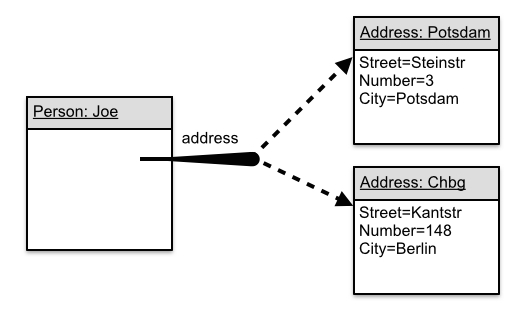
\includegraphics[width=0.5\textwidth]{figures/4_approach/versionAwareReference.png}
    \caption{A Person object with two versions for its address.}
    \label{fig:VersionAwareReference}
\end{figure}

To resolve a path of an object graph as it was at a particular moment..., versions of objects are created and resolved in a coordinated way.
For this, the version-aware references have access to information on which version is currently the one that should be resolved to.
This can, for example, be a global version identifier that corresponds to information stored for each version of a version-aware reference, as shown in Figure~\ref{fig:MoreVersionAwareReferences}.
This example shows a slightly more comprehensive graph that might result from preserving specific versions while changing particular objects.
We have an initial version, \emph{v1}.
In this, a \emph{Company} object is created and that refers to a \emph{CEO} object using a version-aware reference.
The CEO in turn has an address, also referred to via a version-aware reference.
Next, we preserve this version and then, in version \emph{v2}, the same CEO moves to Berlin and, thus, his address gets changed.
Therefore, the version-aware reference to the address of the first CEO knows two different versions of the same address object.
Finally, to reach the situation shown in Figure~\ref{fig:MoreVersionAwareReferences}, we preserve the second version and change the company's CEO in version \emph{v3}.
We can also see that the new CEO also has its own address.
Now, given the knowledge that \emph{v3} is preceded by \emph{v2} and that by \emph{v1}, the version-aware references can resolve to three different development states the runtime was in.
When, for example, changing the CEO turns out to be a mistake, we can re-establish \emph{v2} and with it the old CEO with its address in Berlin as head of the company.
This way, when version-aware references are used consistently for all object relations in a programming runtime, the state of the entire runtime can be set to particular preserved versions.

\begin{figure}[h]
    \centering
    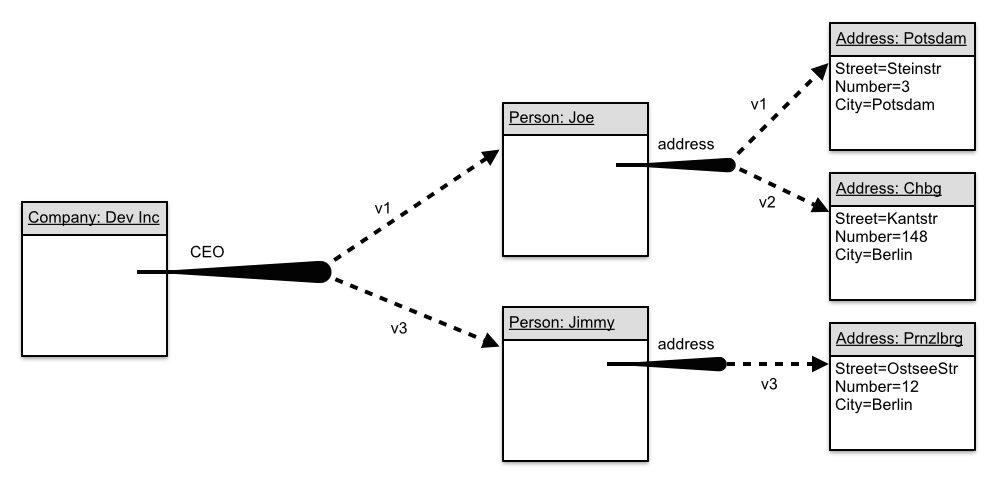
\includegraphics[width=\textwidth]{figures/4_approach/multipleVersionAwareReferences.png}
    \caption{Three versions visible in the version-aware references of a simple object graph.}
    \label{fig:MoreVersionAwareReferences}
\end{figure}

\todo{add code for the path through the object graph}
\todo{add version info (context info) to figures, where necessary}

\todo{add a Figure that shows the three versions of the company object graph separately and incorporate it into the text..}

Which states of the runtime get preserved is not inherent to our approach, but can be different for different use cases. % but also say that versions are created at specific times, specific state preserved (not all situations are recoverable)
Programmers could explicitly preserve versions or the programming system could do this implicitly.
When the programming system is resposible, each manipulating action of a programmer could, for example, yield a new version of the runtime, so programmers can reason about their concrete steps when undoing changes.
Actions that yield new versions could include directly manipulating attributes and composition of graphical elements, editing source code, evaluating do-its, and, for example, clicking buttons of an application.
This way, programmers could also always undo every actions, regardless of whether the action was intended as mere exploration and, thus, the current state protected by a version or whether the action turned out to be inappropriate more unexpectedly.
Using user actions as granularity allows developers to undo and redo the changes associated with specific and rememberable actions.



% transparency of version-awareness / versions

Version-aware references behave transparently, just like a usual reference to the current version of the object would.
They are assigned to variables and get passed around, and, under usual circumstances, programmers do not have to be aware of them.
Firstly, programmers should not be required to adapt their programs to use version-aware references.
Instead version-aware references should be provided consistently by the programming system.
Secondly, there should be no direct references to particular versions of objects.
Programmers should not have to distinguish between version-aware references and direct references, while having both direct references to one particular version and a version-aware reference that always refers to current version could also introduce inconsistencies.


% design implications & rationale

The resulting histories can be fine-grained as for each version only changed objects need to be copied.
Further, creating many versions is not expected to interrupt the programmers workflow as the execution costs of preserving a version is spread: Instead of copying all objects the moment a version should be preserved, objects are only copied when and in the moment they are subsequentely changed.
In general, the approach aims to distribute the cost for object versioning: besides incrementally saving a version, switching the active version is also not interruptive as the version-aware references resolve to versions dynamically and all versions reside as objects in application memory.


This version-aware references allow to change versions without stopping the system.
For this, the version-aware references resolve dynamically to particular versions based on context information.
Only this context information has to be changed to have all references resolve to another version, without updating any of the version-aware references.
Preserving a new version of the runtime also happens incrementally.
Instead of saving versions of all objects that make up the runtime, when the development state is to be preserved, new versions of objects can be created only when objects subsequentely change.
Before such writes the previous object states continue to reflect the current state and can, thus, be read for following versions until written.
This way, as \emph{objects} are copied on writes, versioning happens automatically on the granularity of objects.






% That is, objects are referred to by references that dynamically and transparently choose one particular version of the objects as they were at a particular moment.
% When these references are then used for all mutable objects of a runtime, the entire runtime state can be preserved and re-established.
% 
% Our concrete solution for implementing this in JavaScript and for the Lively Kernel relies on proxies and source transformations.
% Using proxies and source transformations allows a language-level solution for alternative references.
% Versions of objects are also just JavaScript objects and, thus, also in memory.
% The proxies, in this solution, also contain the versions of the object they stand-in for.
% This way, when a proxy, which stands in for all versions of conceptually one object, is no longer referred to from anywhere, all versions of an objects are reclaimed by the ordinary JavaScript gargage collector.









\section{Using Proxies for Version-aware References} \label{sec:APPROACH:2}

% TODO STRUCTURE TODO

% what proxies do / how proxies are used as references/version-aware references

% source transformations to have proxies be used consistently
% garbage collection of proxies and versions

% rationale for using proxies:
% (as opposed to providing alternative references on virtual machine-level: language-level solution as there are many different engines used for executing JavaScript (which would all require implementations of version-aware references to have the Lively Kernel with recovery support for all users. also implementation in JavaScript is easier (especially for a first prototype) and does not have to go through any formal review or standardization process, which language features added to JS engines usually do))


For a concrete solution for the Lively Kernel, we propose to use proxies for version-aware references.
These versioning proxies manage the different versions of an object and can delegate object access to one of these.
The references that usually refer to objects then need to refer to the proxies for these objects instead. 
This is accomplished by returning proxies directly when an object is created.
For this, we transform sources to proxy object literals and constructor functions.
Proxies for functions then return objects always proxied when used as constructors or otherwise to create new objects.
When these proxy-based version-aware references can know the versions of an object and are used consistently to access mutable objects, the proxies only need to know which versions to choose at a given moment and when to copy current versions to preserve particular runtime states.
For this, the runtime is enhanced with a global version identifier representing the current version, which the proxies use to annotate newly proxied objects or new versions of objects with and also to choose the correspondingly annotated versions when accessing proxies.
This then is enough to provide a simple undo/redo for the Lively Kernel.


The proxies required for our solution are virtual-object proxies, proxies that can intercept and response arbitrarily on access.
Such proxies are usually not associated with a particular object or, in our case, version of an object.
When such a fully virtual object proxy is created for an exisiting or new object, the object needs to be just one among potentially many different versions of an object that the proxy might need to forward access to.
The proxies need to be able to intercept and arbitrarily handle all kinds of access transparently.
In fact, the proxies need to fulfill at least three responsibilities:
\begin{enumerate}
    \item They need to know which versions are available for a particular object.
    \item They need to choose one particular version among all available dynamically using context information.
    \item They need to delegate object access transparently to a chosen version.
\end{enumerate}


% TODO: incorporate how version-aware references get resolved into the above sections

% 
% Proxies hold multiple versions of an object.
% They can transparently delegate access to one particular among many versions.
% They are also referred to consistently instead of the object.
% This allows to have and use particular versions of particular objects.
% However, to enable programmers to undo and redo arbitrary changes to the entire development state, our solution needs to preserve and choose versions of all objects in a coordinated way and be able to establish particular versions of the entire runtime instead of just of single objects.
% Our solution to this is declaring versions of the runtime and, then, annotating versions of objects with the version of the runtime they are part of.
% 
% 
% \todo{continue here: write this subsection.. and figure out what details to explain here and which as part of the implementation...}
% 
% 
% global version information: linear: versions with predecessors and successors, maybe with a figure..
% 
% These information are used to decide to which particular versions of objects proxies are to delegate at any moment.
% Given which version of the runtime is currently active, the proxies can choose the corresponding version of the object.
% 
% 
% This way, the proxies transitively all delegate to objects that accurately represent the state of the entire runtime as it was at a particular moment---when the version of the runtime was last active.
% To preserve a development state, the version of the runtime just has to be changed.
% 
% 
% 
% 
% The version of the runtime can be global in JavaScript as JavaScript engines use only a single thread and cooperative scheduling.
% There is, therefore, no way to change which version of each object should be used while a path through an object graph is already partly resolved.




% TODO: subsubsection / paragraph on garbage collection

In our solution, we used the proxies also to hold all versions of the object they stand-in for.
This way, when the proxy is no longer reachable and, thus, eventually garbage collected, all versions of the objects are also collected.
For example, in the following code snippet, there would temporarily exist a version-aware reference---a proxy---connecting the \emph{Person} object to an \emph{Address} object, but the reference gets deleted before a version of the person is preserved:


\iffalse
\begin{verbatim}\fi
\begin{code}[lst:example]{}{float,numbers=left}
    var person = {name: "Lauritz"};
    \\ preserve first version
    person.currentAddress = {street: "Friedrichstrasse",
                         number: "112b",
                         city: "Berlin"};
    delete person.currentAddress;
    \\ preserve second version
\end{code}
\iffalse
\end{verbatim}\fi

That is, the address object is not required to re-establish either \emph{Version 1} or \emph{Version 2} and, thus, nothing should prevent the garbage collector from claiming the proxy for the address object and the address object itself.





% TODO: how to use these proxies to refer to mutable objects / subsubsection or paragraph

% \subsection{Proxies For All Mutable Objects}

% This ensures that references to proxies are used consistently instead of direct references to objects and that such proxies are used for every object.

When proxies are supposed to provide a kind of alternative references, ordinary references that usually point directly to an object now need to point to an object's proxy instead, which then can refer to one or multiple versions of the object.
To have all references refer to proxies instead of actual objects, proxies are created and returned for each new object when objects are created.
The only reference to the actual object---or, more precisely, the initial version of an object---remains inside the proxy, while the reference to the proxy gets passed around instead.
Therefore, all access goes through the proxy and the proxy forwards the access to a particular version of an object.
Also, all references that would usually point to the same object now point to the same proxy, so that proxies provide object identity.
Checks that would usually compare an object with other objects now compare a proxy with other proxies.

For this solution, all expressions that create new objects need to return proxies for those instead.

% TODO: move concrete steps to the implementation, state the following much more abstractly 

% TODO: when/wherever the following is expressed, the three categories should be three similarly named paragraphs after the initial introduction of the categories in the list

% In JavaScript, there are three different ways to create an object: 
% \begin{itemize}
%     \item evaluating literal expressions: e.g. \lstinline|{age: 12}|
%     \item applying constructor functions: e.g. \lstinline|new Person(12)|
%     \item calling specific built-in functions: e.g. \lstinline|Object.create(prototype, {age: 12})|
% \end{itemize}

% We use source transformations to wrap literal expressions consistently into a \emph{proxyFor()} function.
% That function takes an object as parameter and returns a proxy for it.
% Besides objects, arrays and functions are also mutable objects in JavaScript.
% Therefore, we wrap the literal forms of objects, arrays, and functions.
% For exampe, \lstinline{[aPerson, aCompany]} becomes \lstinline{proxyFor([aPerson, aCompany])}.
% 
% In JavaScript, all functions can be constructors and create new objects when called with the \emph{new} operator.
% Functions expressed as function literals already get proxied with the previous source transformations and the proxies we use for version-aware references intercept different object access differently, so proxies for functions can have a specific constructor-behavior that always returns proxies for newly created objects.
% 
% For the functions that create new objects but are built-in and, thus, are not created from literal form, the transformation of literals and proxy behavior is not enough.
% One category of such built-in functions are built-in constructors.
% For example, the built-in data types like objects and arrays can be created by evaluating \lstinline{new Object()} and \lstinline{new Array()}, but also by evaluating just \lstinline{Object()} or \lstinline{Array()}.
% We transform these built-in constructor functions explicity, wrapping each into the proxying function, and also specify the proxies' apply-behavior to also always return proxies.
% Besides these built-in constructors, there are also very specific built-in functions, that we transform separately to specific alternatives.
% One example for such functions is the global \lstinline{eval()} function.
% While the return value of that function also potentially needs to be a reference to a proxy instead of an ordinary object, eval takes arbitrary code which might express an arbitrary object structure and which might, therefore, require multiple references to go through proxies.
% Therefore, in the specific case of eval, we proxy eval's result but in addition also pass the string argument of \lstinline{eval()} through the source transformations before actually providing it for evaluation.



Proxies allow a language-level implementation of alternative references in JavaScript:
Without requiring adaptions to the virtual execution engines, proxies can be inserted to stand-in for objects---so references that usually point directly to objects point to proxies instead---and these proxies can provide versioning information and behavior.
These proxies are, thus, an alternative to using ordinary references to directly refer to objects.
That is, some objects can, potentially, still be referred to directly, while objects that should be versioned should be accessed only though proxies.
In our solution for the Lively Kernel, nearly all objects are only accessed through proxies, except for some particular \emph{root objects} that are not required to be versioned but potentially do refer to other objects via version-aware references.


\chapter{Implementation with Proxies} \label{chapter:IMPLEMENTATION}

% additional TODO: .call + .apply, handle special cases also when functions are arguments these native functions..
% and TODO: [what about all other source transformations..??]

We implemented version-aware references for our approach to object versioning in JavaScript using proxies and source transformations.
This way, our prototype does not require changes to JavaScript engines, but only a certain JavaScript language feature.
In particular, it requires the Direct Proxies\footnote{\url{http://wiki.ecmascript.org/doku.php?id=harmony:direct_proxies}, accessed February 3rd, 2014} as proposed with Version 6 of ECMAScript, the standard that JavaScript follows.
These proxies can implement specific behavior to handle various kinds of access to them.
In our implementation, these proxies are used to delegate all access to a particular version of the object they stand in for.
To have these proxies intercept access to all mutable objects for which versions should be preserved, our prototype uses a combination of source transformations and proxy behavior.
In particular, the moment such mutable objects get created, our proxies get created for the new objects and references to these proxies are returned instead of references to the actual objects.
The proxies then preserve and choose versions of their object corresponding to a global version identifier.
This version identifier effectively declares one particular state of the programming runtime, consisting of those versions of objects that are associated with that runtime state, to be read and written.
Therefore, to change the entire runtime state as, for example, an undo and redo would require only the global version identifier needs to be changed.


\section{Using ECMAScript 6 Direct Proxies}

Our implementation of version-aware references is based on the ECMAScript 6 Direct Proxies.
While these are supposed to stand-in for particular objects, their \emph{targets}, they can also be used as fully virtual objects.
In our case, the proxies represent multiple different versions of an object and do not delegate to any of those by default.
Instead, they choose one of potentially many versions of an object to delegate to dynamically.
Further, the Direct Proxies in our implementation also stand-in transparently for the multiple versions of an object.
That is, the proxies always do behave---except for some specific introspection cases---as if they were a specific version of an object and programmers should not have to be aware about the versioning proxies.

The behavior of the proxies can be specified in \emph{Traps}, methods to specify how exactly specific access to the proxy should be handled, which are bundled in a \emph{Handler} object that is supplied when creating the proxies.
Our implementation of version-aware references using proxies is, thus, defined by our specific proxy handlers that provide the necessary delegation behavior through the traps.
Specific traps are called for specific access. 
For example, when \lstinline{person} is a proxy and \lstinline{person.age} is called, the \emph{get}-trap is called and receives \lstinline{target}, \lstinline{name}, and \lstinline{receiver} as arguments.
In our implementation, the \emph{target} parameter is irrelevant as we use proxies as virtual objects, not to be associated with any particular target object.
The other two parameters, however, are relevant and, for the given example, the \emph{name} would be the string \'age\' and \emph{receiver} would be the proxy for \emph{person} again.
Our proxy handler's \emph{get}-trap is implemented as indicated by the following code snippet, which is, however, simplified in that it leaves out much of the handling of special cases that are due to the shortcomings of the used implementation of Direct Proxies:

\iffalse
\begin{verbatim}\fi
\begin{code}{}{}
get: function(dummyTarget, name, receiver) {

    var version = this.currentVersion();
    
    // proxy meta information and other special cases..
    if (name === 'isProxy') {
    // ...
    if (name === 'proxyTarget') {
    // ...
    
    result = version[name];
    
    return this.ensureProxied(result);
}
\end{code}
\iffalse
\end{verbatim}\fi

First, the current version gets determined using the \lstinline{currentVersion()} function, which is explained in \ref{sec:IMPLEMENTATION:3}.
Then, multiple special cases are handled, including special properties to allow to determine whether a proxy, which otherwise behaves transparently, actually is a proxy or to allow to unwrap the current version from the proxy.
In the simple scenario that we are only reading a property named \lstinline{age} from an object \lstinline{person} all these special conditions fall through.
Instead, the trap reads the property from the current version and returns the result.
The result is passed to the \lstinline{ensureProxied()} function to make sure that mutable objects are proxied.
When a mutable object that is not wrapped in a proxy is passed to this function, the function returns a proxy instead.
This is necessary as, while application-specific objects properties are expected to be proxied, some built-in objects in JavaScript engines refer to their properties directly and not through proxies, but these properties might be required to be proxied to be versioned and to implement version-aware behavior.

Besides the \emph{get}-trap, our proxy handler similarly provides behavior for all other traps, which also delegate to the currently selected version of the object.
The following table \todo{table caption and refer its ref number} provides an overview over the implemented proxy traps:

\begin{table}[h]
\begin{tabular}{|l|l|r|}
\hline
get: function(target, name, receiver) \\ \hline
set: function(target, name, value, receiver) \\ \hline
apply: function(target, suppliedThisArg, suppliedArgs) \\ \hline
construct: function(target, args) \\ \hline
has: function(target, name) \\ \hline
hasOwn: function(target, name) \\ \hline
defineProperty: function(target, name, desc) \\ \hline
deleteProperty: function(target, name) \\ \hline
getOwnPropertyNames: function(target) \\ \hline
getPrototypeOf: function(target) \\ \hline
freeze: function(target) \\ \hline
seal: function(target) \\ \hline
preventExtensions: function(target) \\ \hline
isFrozen: function(target) \\ \hline
isSealed: function(target) \\ \hline
isExtensible: function(target) \\ \hline
enumerate: function(target) \\ \hline
keys: function(target) \\ \hline
\end{tabular}
\end{table}

All these traps fire either when the proxy is accessed with specific JavaScript operators or when it is passed to meta-programming facilities provided by built-in globals\footnote{\url{http://wiki.ecmascript.org/doku.php?id=harmony:direct_proxies\#api}, accessed March 5, 2014}.
For example, the \lstinline{preventExtensions}-trap fires when a proxy is passed to the built-in \lstinline{Object.preventExtensions()} function, which prevents new properties from subsequentely being added to an object.

There currently is no \lstinline{instanceof} trap to intercept the behavior of the \lstinline{instanceof} operator since the Direct Proxies currently do not provide such a trap.
However, the type of an object in JavaScript is defined by an object's prototype chain, which may change at runtime.
So, while the prototype of an object is a property and gets versioned as well, the \lstinline{instanceof} operator does not get trapped and, thus, is not delegated to the current version of the object.
Therefore, this particular object access needs to be handled by a custom \lstinline{Object.instanceof()} function, which implments the semantics of JacaScript's \lstinline{instanceof} operator but does delegate the necessary checks when a versioning proxy gets passed to it.
To exchange all usage of the \lstinline{instanceof} operator with application of this custom function, we transform JavaScript sources before execution.
These transformations change, for example, \lstinline{anObject instanceof SomeConstructor} to \lstinline{Object.instanceOf(anObject, SomeConstructor)}.

The handler object is an ordinary JavaScript object and, thus, can hold arbitrary properties.
Besides providing the trap methods, our proxy handler objects also hold the versions of the represented object.
For this, the proxy handler uses an object as dictionary that associates version identifiers with the different versions of the object.
This version dictionary is used by the handler's \lstinline{currentVersion} function that decides which of the versions should currently be accessed.
Having the handler object hold all the versions of conceptionally one object also takes care of garbage collection.
When a proxy gets garbage collected, all versions get garbage collected as well.

Certain workarounds are required to make our proxy-based implementation of version-aware references work, due to the preliminary status of the proxy implementation.
While the specification of Direct Proxies already progressed from proposal status to being part of the current ECMAScript 6 Draft\footnote{\url{http://people.mozilla.org/~jorendorff/es6-draft.html}, accessed March 5th, 2014}, it is still in draft status and not yet implemented in the JavaScript engines used by the Chrome browser and the Firefox browser.
These two engines currently both implement two different deprecated proposals for the proxies instead of the most recent ECMAScript 6 Draft.
The \emph{harmony-reflect} library\footnote{\url{http://github.com/tvcutsem/harmony-reflect}, accessed February 3, 2014, used version 0.0.11}, however, provides the current API of Direct Proxies for recent versions of both Chrome and Firefox, on top of the implementations of the different deprecated proposal states.
That is, our versioning proxies prinicipally work in both Chrome and Firefox and rely on the \emph{harmony-reflect} shim for this.
However, even with the shim, three issues need to be addressed with technical workarounds that might no longer be necessary once ECMAScript 6 standard gets finalized and fully implemented by the JavaScript engines: 

\begin{enumerate}
    \item Certain built-in JavaScript functions dont handle proxies correctly.
    \item The proxies have to be provided with an actual target, even when implementing virtual objects and consistency checks compare return values of traps to the state of the actual target. 
    \item It is not possible to set the prototype of an object when the current prototype is a proxy due to a bug in Chrome.
\end{enumerate}

Some built-in functions react to proxies with actual errors, return wrong results, or otherwise do not provide the usual functionality.
Therefore, these functions need to be provided with actual objects instead of the proxy.
This is unproblematic for most cases as, given JavaScript's single-threaded and cooperative execution in browser engines, which version of an object is to be used is not expected to change during the execution of a built-in function.
Our implementation provides the current version of an object to these built-in functions through proxy handler traps and patched built-in functions.
The \emph{apply}-trap, called when proxied functions get applied, unwraps all arguments and the \emph{thisContext} object, when the applied function is a built-in functions that does not handle proxies.
This is for example the case for the functions that provide access to the browser's document model.
Further, the \emph{set}-trap sometimes needs to unwrap the assigned value when that value is proxied and gets assigned to slots that cannot handle proxies.
This is for example the case with the \lstinline{onreadystatechange} slot of \emph{XMLHttpRequest} objects.
This particular slot holds functions as callbacks of asynchronous HTTP requests, which, however, do not get called when these functions are proxies.
This is particular case is potentially problematic.
Though JavaScript does get executed with a single thread  using cooperative scheduling by all popular browsers, other concurrent scripts might get executed before a script ends whenever a script is waiting on I/O like, for example, an asynchronous request to finish.
As this---changing a callback function or its properties while waiting on the response---is unlikely, bad programming style as it introduces dependencies to the timing of network I/O, and is through network communication already at the limit of what object versioning can due in general, our implementation currently does not provide a workaround for this specific case, even though we are aware of this potential problem. 
In addition to these behavior implemented in traps, there are also certain immutable types that do not get proxied at all in our implemention as, for example, strings.
However, some methods of, for example, string objects also do not handle proxies correctly and our implementation, therefore, patches those functions to also unwrap proxies before executing the original functions.


\todo{dummytarget: rework the following part..} 
% TODO: dummytarget.. say something about our adaptions to harmony-reflect: no-target flag.. to disable consistency checks of configured properties (frozen..etc)
Instead, as the implementation of the proxies currently requires one particular \emph{target} object even for proxies intended to be virtual objects, the \lstinline{instanceof} operator returns the type of that initial target object.



\todo{Second, proxies as prototypes (relation cant be changed.. traps of proto fire when inheriting object is accessed.. problem is Chrome and only the proto case...)... protoProxy property on objects..}
\todo{maybe explain the design decisions behind the protoID}
% firing proto traps, except when using the new Reflect API, but can't use Reflect.setPrototype in recent Chromes, where Lively runs best..





\section{Returning Proxies For New Objects}

As we use proxies as version-aware references while the JavaScript runtime still only provides ordinary references, references that usually would point to objects directly now need to point to proxies instead. 
References to the same object further need to point to the same proxy for that object.
This is necessary because identity checks will compare proxies instead of objects.
Also because, at least in our implementation, proxies actually hold the different versions of their objects as opposed to looking the objects up in a separate data structure, one particular proxy knows the versions of an object.
Therefore, all references that would normally refer to the object need to refer to the proxy that stands-in for the versions of the objects.
To achieve this, we create proxies immediately for new objects and return the proxies instead of the objects, so a reference to the proxy gets passed around instead of the reference to the actual object, which instead is captured in the versions dictionary of the proxy.

We need to create proxies for all new mutable state, which in JavaScript comprises of objects, arrays, and functions.
JavaScript allows to create these kinds of objects through literal expressions, through constructors, and through built-in functions.
That is, functions are objects and can also have properties in JavaScript.
Constructors can be built-in as, for example, \lstinline{Array} or literal functions.
Both create new objects when applied with the \lstinline{new} keyword, however built-in constructors also return new objects when applied without the \lstinline{new} operator.
Other built-in functions are, for example, \lstinline{eval} or \lstinline{Object.create(..)}.
To actually create and return proxies from all these three different ways to create objects, our implementation transforms sources before execution.
The built-in functions could be overwritten globally to return proxies for the new objects, but our implementation of object versioning also uses these built-in data types internally.
Additionally, at the time of writing, some JavaScript engines do not allow to overwrite particular built-in functions, while we want our implementation of object versioning to work in every JavaScript engine that supports ECMAScript 6 Direct Proxies.
Therefore, we transform specific literal expressions and specific built-in functions, while custom constructors return proxies through particular proxy trap behavior.

The source transformations for introducing our proxy-based version-aware references wrap the original expressions into the \lstinline{proxyFor} function, which returns a proxy for an object.
The transformations of literal objects, arrays, and functions are shown by example in following table.

\begin{center}
    \begin{tabular}{| l | l | l | l |}
    \hline
    Type & Original code & Transformed code \\ \hline
    \emph{Objects} & \lstinline|{name: 'James', age: 24}| & \lstinline|proxyFor(name: 'James', age: 24)| \\ \hline
    \emph{Arrays} & \lstinline|[person1, person2]| & \lstinline|proxyFor([person1, person2])| \\ \hline
    \emph{Functions} & \lstinline|function (a, b) {..}| & \lstinline|proxyFor(function (a, b) {..})| \\ \hline
    \end{tabular}
\end{center}

Besides straightforward wrapping of literal objects, literal arrays, and function expressions, the source transformations also needs to handle function declarations and accessor functions.
Function declarations are named functions, where the name is available for recursion in the function itself, but also makes the function accessible by the name in the surrounding scope.
For this reason, the function declaration get transformed to function expressions that are assigned to matching variable names.
This way, \lstinline|function funcName(..) {..}| becomes \lstinline|var funcName = function funcName(..) {..}|.
In addition, because function declarations get hoisted in JavaScript, the source transformation moves the results of transforming function declarations to the beginning of the defining scope, while the order among function declaration is preserved.
Accessor functions are functions that are executed instead of ordinary read or write access to properties.
The following example snippet shows the definition of a \lstinline{person} object, where two accessor functions allow reading and writing \lstinline{person.age} while the value is stored under a different name: \\
\iffalse
\begin{verbatim}\fi
\begin{code}{}{}
var person = {
    __age: 0,
    get age() {
        return this.__age;
    },
    set age(val) {
        this.__age = val;
    }
}
\end{code}
\iffalse
\end{verbatim}\fi

Wrapping the two accessor functions in-place into \lstinline{proxyFor} functions does not yield valid JavaScript code.
Therefore, the source transformations wrap object literals with accessor functions into anonymous functions that are directly applied, create the objects first without accessor functions, and explicitly define the accessor functions using \lstinline{Object.defineProperty}.
That is, the presented example with accessor functions would be transformed to the following code: \\

\iffalse
\begin{verbatim}\fi
\begin{code}{}{}
var person = function() {
    var newObject = lively.proxyFor({
        __age: 0;
    });
    Object.defineProperty(newObject, "age", {
        get: lively.proxyFor(function age() {
            return this.__age;
        }),
        set: lively.proxyFor(function age(val) {
            this.__age = val;
        }),
        enumerable: true,
        configurable: true
    });
    return newObject;
}();'
\end{code}
\iffalse
\end{verbatim}\fi

Similar to the wrapping of object literals without accessor functions, arrays, and function expressions, the source transformation also wraps specific built-in functions into calls to the \lstinline{proxyFor()} functions.
For example, \lstinline{Array(100)} becomes \lstinline{proxyFor(Array(100))}.
As every call to such built-in objects is transformed in this way, the same Object---in this case the \lstinline{Array} function---gets passed to the \lstinline{proxyFor} function multiple times.
To nevertheless return the same proxy and, therefore, the same identity, we use a map that associates objects with their proxies.
This \emph{Proxy Table} is a weak-key map and does not prevent neither objects nor proxies from being gargabe collected.
Therefore, the following statement returns true for an arbitrary object \lstinline{obj}: \lstinline{proxyFor(obj) === proxyFor(obj)}.

When objects get created through applying functions with the \lstinline{new} operator, the new objects also need to be proxied.
However, as the functions are already proxied through source transformations of function literals and the built-in \lstinline{Function} constructor, our implementation does not transform the applications of the \lstinline{new} operator, but uses the \emph{construct} trap to return proxies from constructor applications.
The last line of code of the \lstinline{construct} function of our proxy handler is therefore: \lstinline{return this.ensureProxied(newInstance)}.
This is also true for the \emph{apply} trap, because, for example, the \lstinline{Array} and \lstinline{Object} functions also create objects when called without the \lstinline{new} operator and, for example, the built-in function \lstinline{Object.create(proto)} also returns a new object.
In fact, with our proxy handler the \emph{get}-trap also makes sure to return always proxy in this fashion.
So, wrapping \lstinline{Object} is enough to have \lstinline{Object.create(proto)} return a proxy: \lstinline{Object} transforms to \lstinline{proxyFor(Object)}, while getting the property returns a proxy for the \emph{create} function, and applying that in turn also returns a proxy.

The implementation of source transformations uses \emph{UglifyJS}\footnote{\url{http://github.com/mishoo/UglifyJS2}, accessed March 12, 2014} for parsing and AST transformations.
UglifyJS parses without using JavaScript exceptions for backtracking and, therefore, does not interfere with debugging.
In addition, UglifyJS also supports Source Maps \todo{footnote with url to Source Maps necessary..}, which allow to view and debug the original code with the browser's developer tools, even though the transformed code is executed.



\section{Providing Simple Global Versions for Undo and Redo} \label{sec:IMPLEMENTATION:3}

JS execution: single-threaded, cooperative scheduling 

\begin{itemize}
    \item global versions, linear versioning, data structure is an version object with a predecessor and a successor
    \item copy-on-write for versions of objects (set-trap, apply-trap for some array methods), shallow copy
\end{itemize}


However, some additional logic is required to update state that is not part of the runtime state as, for example, the HTML document presented by browsers.


The version also may have a predecessor and a successor.
This way, for undo and redo the current version of the runtime only has to be set on the predecessor or the successor.
Preserving the predecessor also allows to preserve versions of objects only on writes as, when objects have not changed in versions, the first available previous version of the object can be read.

% Besides this copy-on-write optimization, another optimization would be to not copy objects completely, but to only store changes.
% this could, for example, also apply prototypical inheritance to have versions that delegate to previous versions and only express the differences between versions.

The association proxies associate all available versions of an object with a version of the runtime.


When a proxy is created for an object, the object is preserved as the version of the object that belongs to the current version of the runtime.
On writes, the proxies copy the latest version of the object and then do the write on the copy instead.
The copy gets marked with the identifier of the new version of the runtime.
When the proxies now choose a particular version of the object they stand-in for, they all use the version associated with the current version of the runtime or of a previous versions.


\begin{itemize}
    \item source transformations enabled right after the object versioning code, i.e. the implementation of the proxies and the source transformation, which are both themselves implemented using ordinary javascript code, gets loaded. by patching the eval that is used for evaluated modules that get loaded with an eval(transformSource.. so modules are not versioned, but classes / layers / traits are.. e.g. a class is versioned, so in different versions there might be different class-side state... so, for example, modules are currently in our implementation the roots of the version-aware reference graphs that prevent garbage collection, 
\end{itemize}


\begin{itemize}
    \item undo / redo implementation, example situation
    \item redraw of the world as DOM objects / DOM relations are not part of the object versioning in JavaScript: DOM redrawing on undo / redo: DOM is out of versioning scope, doesn’t use version-aware references, has to be changed / redrawn on undo/redo explicitly
    
\end{itemize}








\section{Limitations of the Implementation}




% \subsection{Limitations for Concurrent JavaScript}


single-threaded and cooperative scheduling, but setTimeout / setInterval... stop asynchronous actions from following versions when undoing... source transformations, which scripts belongs to which version


% \subsection{Limitations in the Execution Environment}

\begin{itemize}
    \item  the proxies are not fully implemented in all browsers, yet, and some built-in browser tools for developers also do not support them entirely.
    only works in recent Chromes, with experimental JavaScript / or Firefox (without adaption)... ECMAScript 6 Direct Proxies not yet fully implemented, not yet stable..
.. own adaptions to the shim library, to bridge the gap between the current version of the shim and information from the Spec draft (pass null for the target of a proxy)... fully virtual objects vs. consistency checks.. adapted library to fit spec draft (pass null as target of a fully virtual object, then no trap-return-value-consistency-with-target checks)
\end{itemize}
    

% \subsection{Usability: Impact on Debugging}

\begin{itemize}
    \item adds lots of low-level frames, dev tools don’t handle proxies well (hovering, labels, stepping into), but we have at least source maps, so developers can debug the original code and not the result of our source transformation
    \item debugging: interference with Chrome's developer tools, which don’t handle proxies well (hovering, labels, stepping into)
\end{itemize}


Besides impacting code execution, the current implementation of object versioning for Lively also  with certain programming tasks.
Though the version-aware references should be transparent to programmers, in the current proxy-based implementation proxies show during debugging.
However, the developer tools show the original source code, despite the implementation's transformations of the sources.

Nevertheless, our implementation is functional and integrated with Lively.
It allows programmers to undo and redo changes and is publicly available\footnote{\url{http://github.com/LivelyKernel/LivelyKernel/commit/858aca8c5ac0f203061823f463fda9b434131636}}.

\chapter{Evaluation} \label{chapter:EVALUATION}

We evaluated our implementation of version-aware references in terms of functionality and practicability, as presented and discussed in this chapter.

Regarding functionality, we evaluated whether our proxy-based version-aware references behave like particular versions and whether they allow to preserve and re-establish versions of the development state of the Lively Kernel.

Regarding practicability, we evaluated the impact of proxy-based version-aware references on both memory consumption and execution speed.

For the tests, we used a standard benchmark suite and the Lively Kernel.


\section{Test Setup}

We tested our implementation with a standard JavaScript benchmark suite, the Lively Kernel, and a particular machine configuration, as described in this section.

\subsection{The Octane JavaScript Benchmark Suite}

% what?
We used the \emph{Octance} benchmark suite\footnote{\url{http://code.google.com/p/octane-benchmark/}, accessed February 3, 2014, at version 26} to test both the behavior and performance overhead of our alternative references.
Octane is a general JavaScript benchmark suite that consists of eight benchmarks.
It does not test JavaScript's language features systematically, but is a suite of real programs such as the \emph{DeltaBlue}\cite{FreemanBenson1990ICS} constraint solver.
These JavaScript programs make, however, use of many important language features, including primitive data types, operators, built-in functions, functions, objects, and prototypical inheritance.
Octane is also used in measuring the performance of \emph{v8}, the engine used by both the Chrome browser and Node.js, and is even part of v8's official source code repository\footnote{\url{http://v8.googlecode.com/svn/}, accessed April 23, 2014, at revision 20901}.

% why?
We decided to use the Octane suite for two reasons.
First, it covers many JavaScript language features and seems to be a benchmark suite that is widely in use.
Second, it is used particularly by the Chrome browser's JavaScript engine and Chrome is also the browser we used for developing and testing our implementation.


\subsection{The Lively Kernel System}

% what?
We continuously tested our system with the Lively Kernel.
We integrated our approach with version 2.1.3 of the Lively Kernel and, in particular, used the commit ba726ddca08df66b775e904366cdcbd76c4920f6\footnote{\url{http://github.com/LivelyKernel/LivelyKernel/commits/ba726ddca08df66b775e904366cdcbd76c4920f6}, accessed February 17, 2014} as starting point for our changes.
The version we used for all experiments described in this section is fc6f3b7e7e75cf3f866a8e5eb5899d65a5530654\footnote{\url{http://github.com/LivelyKernel/LivelyKernel/commits/fc6f3b7e7e75cf3f866a8e5eb5899d65a5530654}, accessed February 17, 2014}.
This version of the Lively Kernel can transform most of the Lively Kernel's code to insert proxies for mutable objects.
In particular, the versioning system is loaded right after loading Lively Kernel's module system.
Thus, enabling the versioning system excludes the Lively Kernel's extensions to the built-in JavaScript types, its bootstrap logic, and its module system, but includes everything loaded thereafter, including all modules and classes of the Lively Kernel.

% why?
We tested our implementation with the Lively Kernel for multiple reasons.
First, the Lively Kernel is a large JavaScript application that makes use of many features of both the JavaScript language but also the browser as particular host environment.
That is, it makes use of not only most of the features described in the language specification, including the language's standard library, but also much of the additional built-in functionality of the browser, which, for example, includes the built-in functions to manipulate the HTML document.
Second, the main goal of the presented work is to provide object versioning for the Lively Kernel.
Thus, we are particularly interested in evaluating our implementation with the Lively Kernel.


\subsection{Test Machine Configuration}

% what?
All tests and measurements were done on a Macbook Air with an 2 GHz Intel Core i7 and 8 GB main memory, using Mac OS X 10.9.1, and the most recent stable release of the Chrome browser on February 18, 2014, which was version 32.0.1700.107.

The presented measurement results were averaged over five runs.

% why?
We used Chrome for all experiments as the Lively Kernel currently works best in Chrome.







\section{Functionality: Versions of the Lively Kernel Runtime} \label{sec:DISCUSSION:1}

We tested whether the version-aware references forward to particular versions correctly both with benchmarks and with the Lively Kernel, as described in this section, and did this continuously during the implementation of our approach.

\subsection{Testing with Benchmarks}

We ran the Octane benchmark suite to test the functionality of our implementation.

\paragraph{Method}
% what was done?
We transformed the Octane benchmarks with our source transformations, executed the resulting code, and then checked for JavaScript errors and compared the results of running the transformed benchmarks to their usual results.\\
% why / to test what?
We did this for to test two aspects.
First, to test whether our source transformations yield syntactically correct JavaScript code for the benchmarks.
Second, to test whether the proxy-based implementation of version-aware references, inserted by the source transformations, allows to run the benchmarks without errors and with the same results as when the benchmarks are executed without our implementation.


\paragraph{Results}
All benchmarks in this suite run without errors and return the same results as when executed without any source transformations.
That is, at least for these tests, our source transformations produce working source code and our proxy-based version-aware references behave as the object versions they stand-in for.
The benchmarks and, in particular, the \emph{DeltaBlue} benchmark revealed a problem with using proxies as prototypes of objects, which we reported to the \emph{harmony-reflect} repository\footnote{\url{http://github.com/tvcutsem/harmony-reflect/issues/18}, accessed April 23, 2014} and which turned out to be an issue with the \emph{v8} JavaScript engine itself\footnote{\url{http://code.google.com/p/v8/issues/detail?id=2804}, accessed April 23, 2014}.
We virtualized the prototype relation among proxies as workaround for this problem in our implementation, but the issue was subsequentely fixed, rendering the implemented workaround redundant.

\paragraph{Discussion}
The proxies, which implement version-aware references, behave like the respective versions of objects in the situations exhibited in the benchmarks.
While these benchmarks do not test JavaScript's features systematically, they cover a range of language features.


\subsection{Testing with the Lively Kernel}

We tested whether the Lively Kernel loads and works as expected when our version-aware references are used.

\paragraph{Method}
% what was done?
We transformed the JavaScript modules of the Lively Kernel at load-time to test whether it loads and works as expected with our versioning system.
We further tested whether the version-aware references and the linear global undo/redo allow to preserve and re-establish versions of the Lively Kernel's JavaScript runtime in practice.
Here, we tried multiple simple example scenarios, including to undo changes to the state and behavior of basic morphs, to morph compositions, and to the state of more complicated graphical applications as, for example, text editors and developer tools.\\
% why / to test what?
With this, we tested that the source transformations yield valid JavaScript code for the modules of the Lively Kernel, that the version-aware references delegate correctly to the versions of objects they stand-in for in Lively, and that the version-aware references are used consistently for all mutable objects.


\paragraph{Results}
The Lively Kernel loads when all of its modules are transformed to use version-aware references.
Further, most of its basic functionality works as expected and we were able to preserve and re-establish runtime states of multiple examples.
However, not all functionality works as expected and we were, thus, also not able to re-establish all preserved states. 
This way, we also learned about the issues of the current state of ECMAScript 6 Direct Proxies in Chrome and implemented the workarounds described in Section~\ref{sec:IMPLEMENTATION:4}.

\paragraph{Discussion}
While most of the tested functionality of the the Lively Kernel---including the entire bootstrap process, rendering graphical objects, loading parts from the Lively Kernel's Parts Bin, and using the Lively Kernel's halo controls---work as expected with version-aware references, certain functionality of the Lively Kernel is not yet working correctly or even yields errors.
The remaining issues here are expected to be problems related to built-in JavaScript functions that do not handle proxies correctly.
Our implementation already unwraps proxies for many built-in functions, as explained in \ref{sec:IMPLEMENTATION:4}, but the configuration appears to currently not cover all problematic built-in functions, yet.
However, the used proxies are still an experimental JavaScript feature in Chrome, not yet fully supported, and we expect these issues not to be problems anymore once the proxies get fully implemented by JavaScript engines.
Further, the current implementation already allows to use many features and re-establish many development states of the Lively Kernel.




\section{Practicability: Additonal Memory Consumption} \label{sec:DISCUSSION:2}

We measured the memory overhead of just the version-aware references, without preserving any version, and also present the memory used when multiple versions of a small example scenario are preserved.

\subsection{Memory Overhead for Version-aware References}

The version-aware references have an impact on memory consumption that has to be practical.

\paragraph{Method}
% what was done?
We measured the memory consumption of an empty Lively world when loaded with and without source transformations and, thus, version-aware references.
In this experiment, we did not preserve any versions of the development state.\\
% why / to test what? 
This way, we only measure the overhead of the proxy-based version-aware references themselves as each of those refers to only one version---the original objects, which are present both with version-aware references and without.
We decided to load an empty Lively Kernel world to measure the overhead in a minimal runtime, while expecting the overhead to grow linearly with the number of proxied objects.

\begin{figure}[h!]
    \centering
    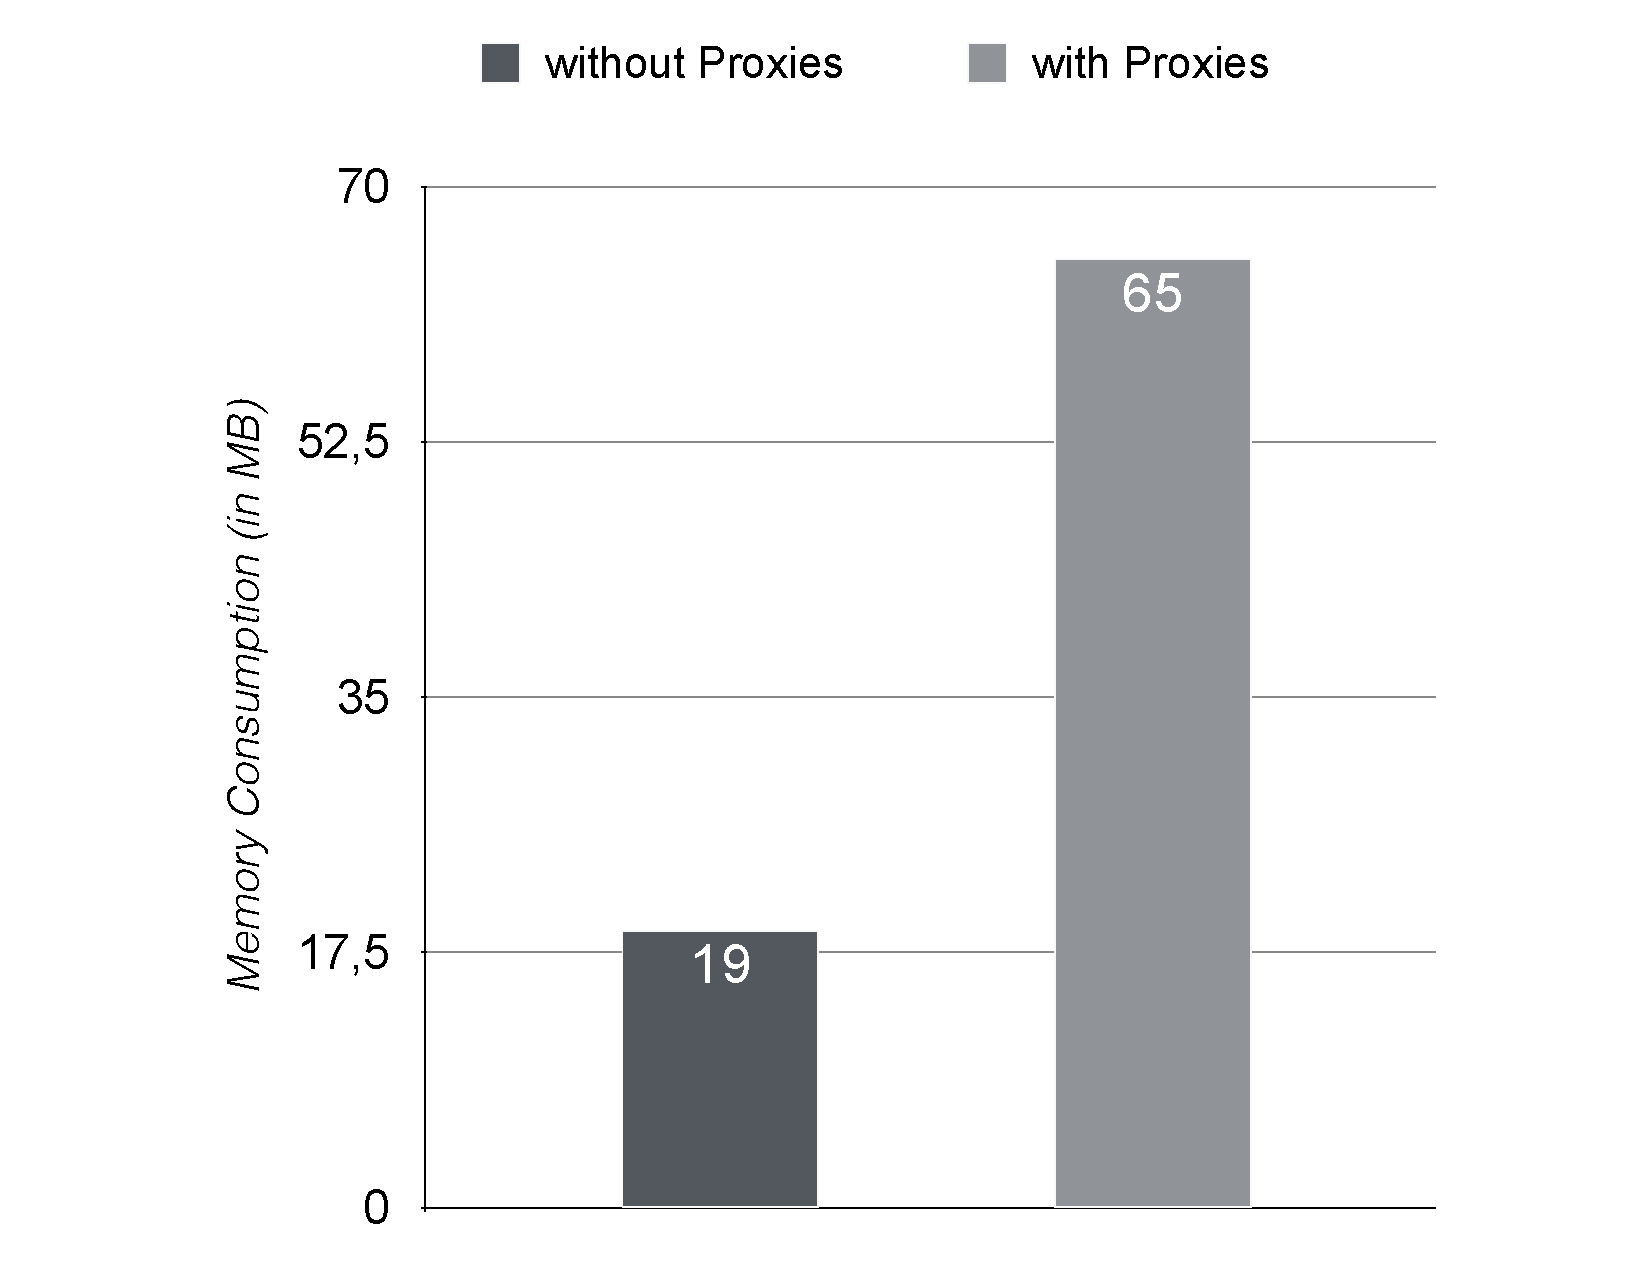
\includegraphics[width=\textwidth]{figures/6_evaluation/1_memoryOverhead.pdf}
    \caption{Memory consumption when starting a Lively Kernel world with and without proxies.}
    \label{fig:MemoryOverheadForReferences}
\end{figure}

\paragraph{Results}
As shown in Figure~\ref{fig:MemoryOverheadForReferences}, loading an empty the Lively Kernel world requires three times more space with proxies than without proxies.

\paragraph{Discussion}
Even without preserving multiple versions of any object, the system requires more space when loaded with versioning proxies.
The system uses a proxy for each created mutable object and all references that would usually refer directly to the object refer to the proxy instead.
These proxies require additional space: Each proxy comprises of at least an internal proxy object, a proxy handler object that implements the proxy's behavior, and an ordinary JavaScript object as dictionary for all available versions of the object the proxy stands-in for.
The memory overhead increases linearly with the number of objects accessed through proxies.
While the system creates proxies for most objects, it does not use proxies for all objects.
In particular, it does not create proxies for objects present before our implementation of object versioning is loaded, including all objects used by the versioning implemenation itself.
We expect the number of objects that are excluded from versioning to be relatively stable, while all additional objects created at runtime will be accompanied by proxies.
Currently, the proxies are not optimized to consume as little space as possible.
Two improvements of the current implementation would be to not create a versions dictionary as long as a proxy stands-in for only one version and to have the proxy handlers of all our proxies share their behavior.
The memory overhead, however, does not appear to be problematic at the moment.


\subsection{Memory Usage for Preserving Versions}

Besides the memory required for the proxies, there is also memory required for preserving multiple versions of the runtime.
Although we expect the memory usage for versions to be highly dependent on the differences between preserved states, we still present a simple example scenario here.

\paragraph{Method}
% what?
To measure how much memory is required for preserving versions of the runtime state, we measured the memory consumed at three different moments in a simple scenario, which are highlighted as \circnum{1}, \circnum{2}, and \circnum{3} in Figure~\ref{fig:MemoryOverheadForVersions}.
The memory measured is not limited to the memory required for versions, but is instead the memory used by the entire JavaScript runtime.
In particular, we did the following:
\begin{enumerate}
    \item We measured the memory consumed for the state \circnum{1} and then commited the version of the runtime.
    \item We changed the state to be state \circnum{2}, measured the memory again, and commited that version.
    \item We changed the state to be state \circnum{3} and measured the memory again.
\end{enumerate}

\begin{figure}[h!]
    \centering
    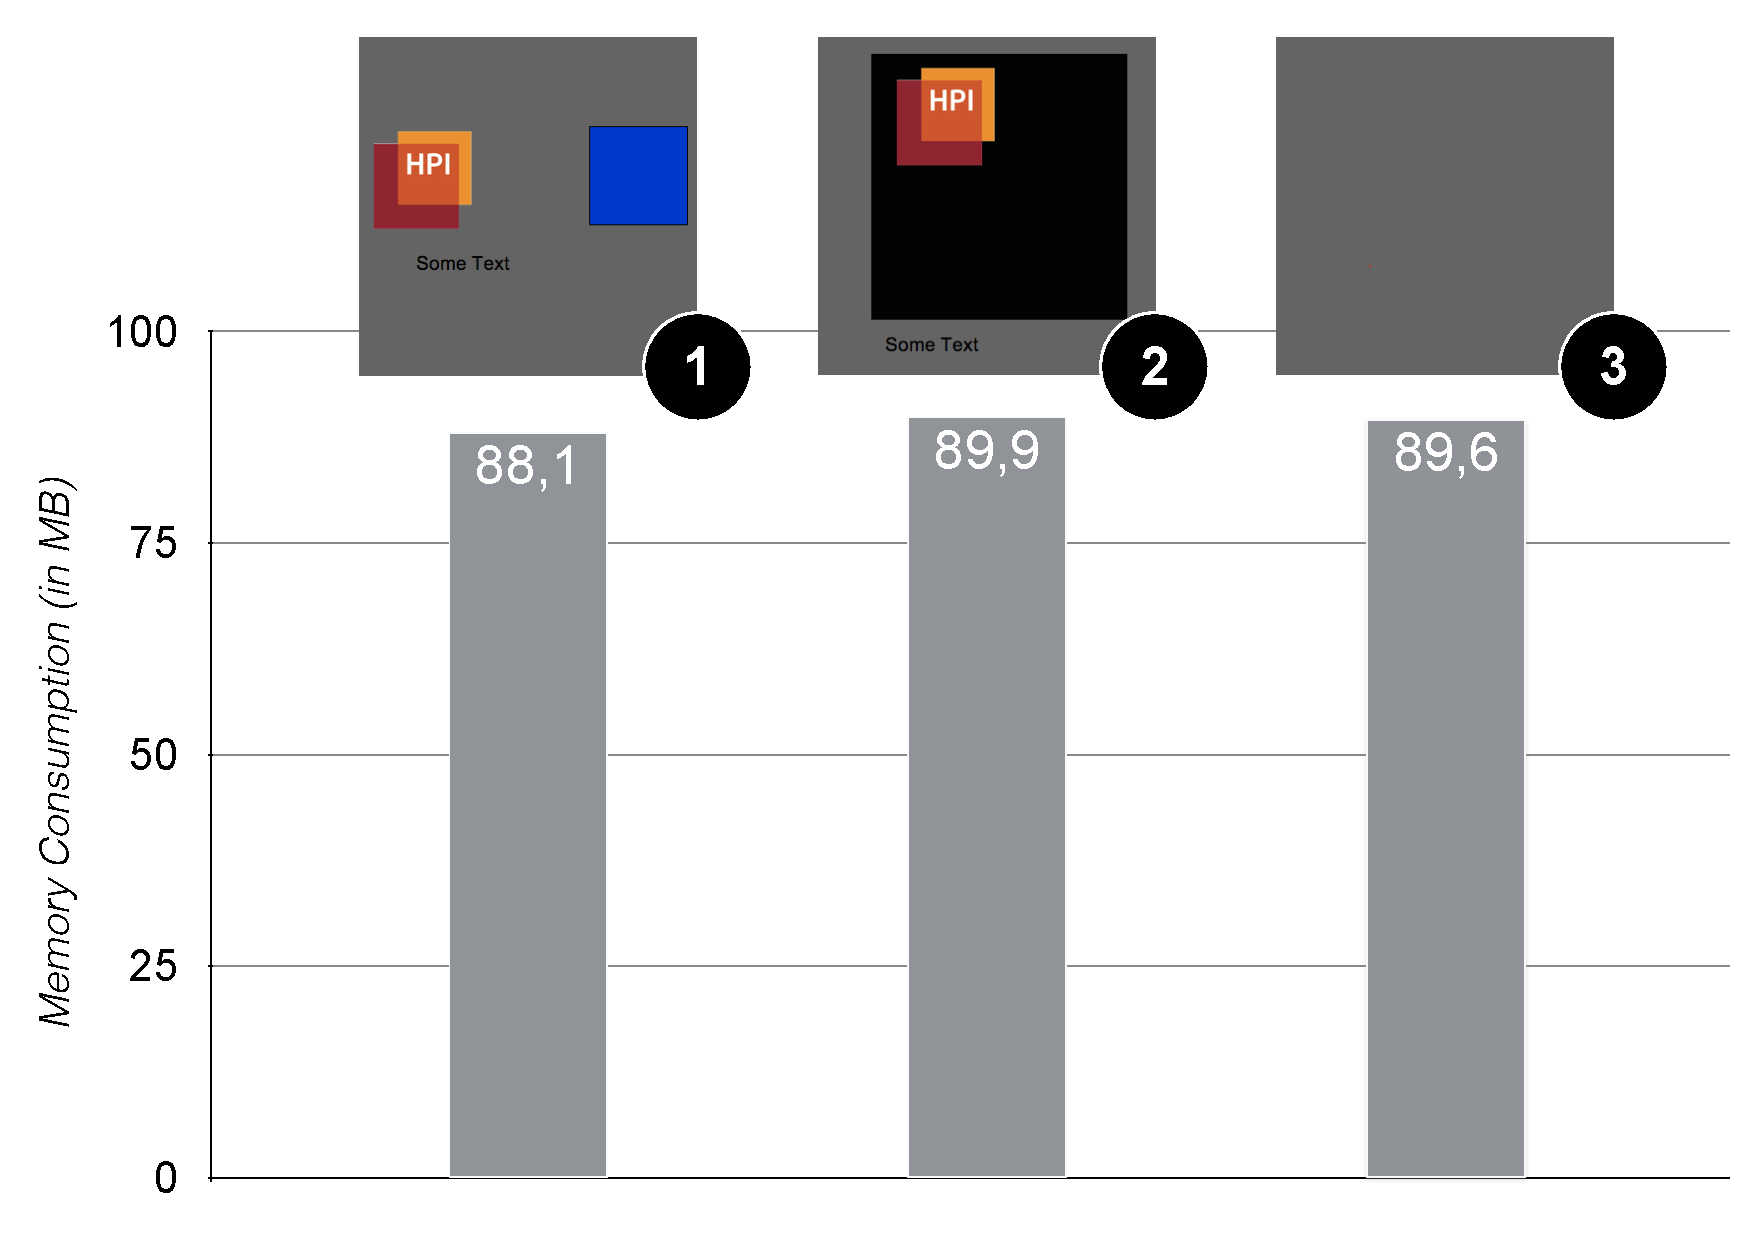
\includegraphics[width=\textwidth]{figures/6_evaluation/2_memoryForVersions.pdf}
    \caption{Memory consumed by the same runtime at three different moments in time, after preserving the previous states.}
    \label{fig:MemoryOverheadForVersions}
\end{figure}

\paragraph{Results}
As shown in Figure~\ref{fig:MemoryOverheadForVersions}, the memory consumption is not very different for the three situations.
The second state required the most memory for the JavaScript runtime, while the memory consumption of the third state is in-between the first and the second.
That is, in this example, the space required for preserving the two states of the morphic objects is insignificant to the space already required for running a Lively Kernel world.

\paragraph{Discussion}
Our implementation does not copy all objects for each version, but only creates copies when objects subsequentely change, effectively storing only the differences between runtime versions.
Therefore, the memory required for preserving versions of the runtime depends on how objects change compared to the predecessor version.
Except for not visible objects created due to mouse interactions, the state \circnum{2} consists of the same objects as state \circnum{1}, but holds multiple versions of the state of the involed morphs and, therefore, the memory footprint increases, but only slightly.
The memory required for the entire JavaScript runtime---not only for preserving versions---does not always increase as there are also temporary objects that are not preserved with any version.
Such temporary objects include the state of JavaScript objects that represent HTML document elements.
These objects can be derived from preserved morph states and, thus, do not have to be preserved.
For this reason, it does not seem odd that state \circnum{3} requires less memory than state \circnum{2}, even though from the third state both previous states can be re-established.\\
\emph{In summary}, the memory overhead for preserving different versions of the runtime does not increase exactly linearly with the number of versions and does not only depend on how many objects are part of the versioned states, but instead highly depends on the differences between preserved versions.



\section{Practicability: Impact on Execution Speed} \label{sec:DISCUSSION:3}

We measured the overhead the proxies impose on the execution of benchmarks and certain functionality of the Lively Kernel.
A discussion of the results follows at the end of this section.


\subsection{Measuring Benchmarks}

The Octane benchmark suite shows how the proxies currently slow down a variety of different JavaScript programs, while two microbenchmarks show the specific cost of using the proxy-based version-aware references.

\subsubsection{Octane Benchmark Suite}

Measuring the Octane benchmark suite highlights how the execution of eight JavaScript programs is affected by the proxies.

\paragraph{Method}
We ran the Octane benchmarks\footnote{Note: We reduced the input size to the Splay benchmark by an order of magnitude to prevent the browser from prompting for user input during the benchmark's execution. The prompt is triggered due to the long time required to run the benchmark. It cannot be disabled and would influence the benchmark result.} with and without previous transformation of the benchmark code and, therefore, with or without version-aware references.
The source transformations for this were done separately and are not reflected in these results.

\begin{figure}[h]
    \centering
    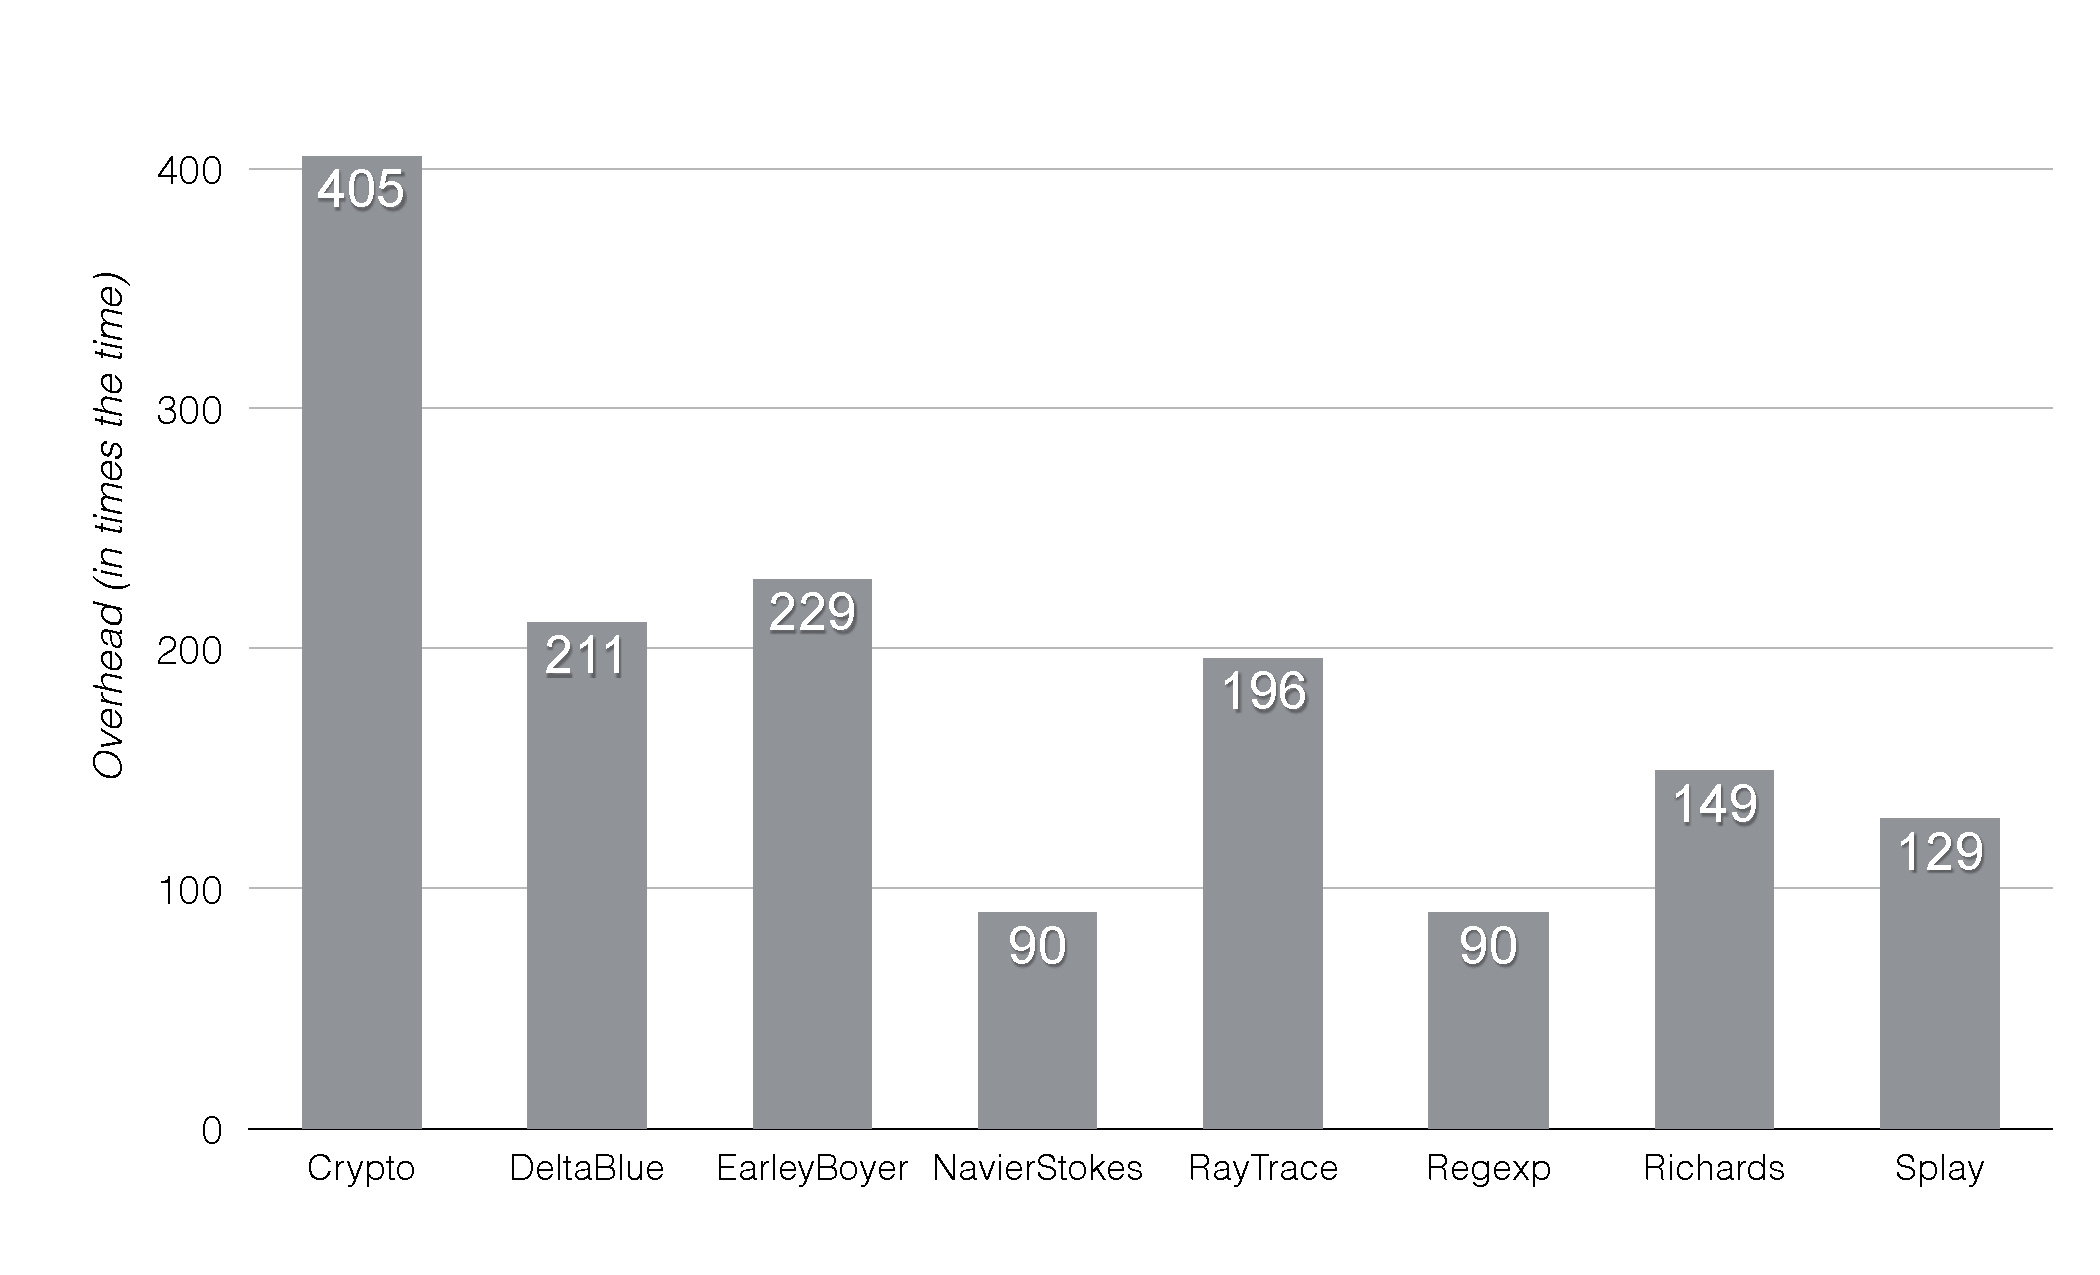
\includegraphics[width=\textwidth]{figures/6_evaluation/3_executionOverhead.pdf}
    \caption{Execution overhead for proxy-based version-aware references compared to ordinary JavaScript references.}
    \label{fig:ExecutionOverhead}
\end{figure}

\paragraph{Results}
Figure~\ref{fig:ExecutionOverhead} shows how much more time the benchmarks take when their source is transformed before execution and references are, therefore, version-aware.
Executing the benchmarks takes between 90 and 405 times longer with version-aware references than without.
On average the slowdown of a single benchmark is, thus, a 187.5 times.


\subsubsection{Microbenchmarks}

We implemented microbenchmarks to analyze the overhead the proxies impose on resolving references---the time proxies take to forward access to a particular version.

\paragraph{Method}
In the first setup, we resolved a reference between two objects a million times, where the reference is either an ordinary reference or a proxy-based version-aware reference.
In the second setup, we exchanged the proxy-based version-aware reference with a standard proxy without providing a handler object.
In this case the proxy falls back on the default proxy behavior, which is forwarding to a single target and which we regard as a minimal overhead for reasonable proxy behavior. 

\paragraph{Results}
In the first setup, the microbenchmark takes three orders of magnitude more time when using the version-aware references: instead of on average 10 milliseconds the test requires on average about 11000 milliseconds to finish.
In the second setup, the difference is an order of magnitude less: with a direct reference the benchmark still requires around 10 milliseconds, while the benchmark requires requires close to 2000 milliseconds with a proxy as connection between both objects.
That is, even the default proxy behavior slows down the microbenchmark close to 200 times.



\subsection{Measuring the Lively Kernel}

We measured the overhead of a few typical user interactions and also how much longer it takes to load a simple Lively Kernel world.

\subsubsection{Typical Lively Kernel Interactions}

As our goal is to provide recovery support for development in Lively Kernel, the impact on typical interactions is especially interesting as it directly experienced by developers.

\paragraph{Method}
% what?
We measured the overhead for typical user interactions in the Lively Kernel by comparing the time three interactions take when using proxies and when not using proxies, from the time of the user event until the single-threaded JavaScript engine becomes responsive again.
The three typical interaction we chose investigate are: bringing up the halo buttons on a particular morph, opening the world's menu, and opening the Lively Kernel's System Code Browser.\\
% why?
We chose these three interactions as they are expected to be among the more impacted interactions compared to, for example, interactions that are more browser-supported and less reliant on JavaScript execution such as dragging elements around the screen.
All three interaction trigger code from multiple different modules, including event handling code, rendering code, and tool-specific code.

\begin{figure}[h]
    \centering
    \includegraphics[width=\textwidth]{figures/6_evaluation/4_LivelyInteractionsOverhead.pdf}
    \caption{Execution overhead for selected user interactions in the Lively Kernel.}
    \label{fig:LivelyInteractionsOverhead}
\end{figure}

\paragraph{Results}
Figure \ref{fig:LivelyInteractionsOverhead} shows the results, which are comparable for all three interactions.
Each of these interactions takes on average 43 times the time when triggered after the system's was loaded with proxies.



\subsubsection{Loading a World in the Lively Kernel}

Another performance-related question specific to the Lively Kernel is how long it takes to load a world.

\paragraph{Method}
We measured how long it takes to load a specific Lively Kernel world both with and without source transformations and, thus, proxies.
Loading a world includes requesting the required modules from the Lively Kernel's server, client-side code to resolve dependencies among modules, evaluating all loaded modules, and deserializing a the Lively Kernel world.
Additionally, in case version-aware references should be used, the sources of all modules also are transformed while loading a world.

\paragraph{Results}
The overhead of loading a world with object versioning is a factor of around eight for loading a world: instead of around 4 seconds, the user would have to wait around 32 seconds until the requested the Lively Kernel world reacts on user interactions.




\subsection{Discussion of the Execution Overhead}

The execution overhead of the current implementation of version-aware references does not appear practical.
The current implementation slows down the JavaScript execution considerably: 

\begin{itemize}
    \item the Octane benchmarks need two to three orders of magnitude more time to finish
    \item the examined user interactions in the Lively Kernel take two orders of magnitude more time
    \item direct comparisons of resolving version-aware references and direct references in a microbenchmark show a slowdown of four orders of magnitude
\end{itemize}

While object versioning could be used to provide the undo/redo of a specific application, it is primalary itented to support development and similar explorative tasks.
That could, conceivably, be an argument for providing object versioning only during development, not when programs are only in-use and should run at full speed.
However, besides having the disadvantage of introducing distinct usage modes, this still requires the version-aware references to resolve fast enough to not impede development significantly, which they currently do not yet do.

We gained the impression that only one order of magnitude is due to the specific proxy behavior, while most of the overhead can be ascribed to using the Direct Proxies as currently available in the Chrome browser.
The proxies are part of an ECMAScript specification that has not yet been finalized and completely implemented by the JavaScript engines.
As explained in Section~\ref{sec:IMPLEMENTATION:1}, the proxies are currently also implemented using a library that relies on an experimental implementation of a previous, deprecated draft of the proxy specification.

Similar behavior forwarding as provided by the proxy handlers could also be implemented in JavaScript, using source transformations and ordinary JavaScript functions.
Instead of using an actual proxy for an object, we could have references point to an ordinary JavaScript object and implement the handler behavior in an ordinary JavaScript function, to be used through further source transformations: instead of \lstinline{obj.prop} the system would execute code similar to \lstinline{get(obj, \"name\")}, where the \lstinline{obj} could still be only a stand-in for many different versions, while \lstinline{get} could implement the behavior previously implemented by respective the proxy trap.
Measuring the performance of such a simple indirection results in a much lower performance overhead for the previously described microbenchmark setup:
it only takes twice the time to read a property from a specific target with a \lstinline{get}-function when compared to reading a property directly.

All this---the experimental status of the proxy implementation, the high cost of proxies even when used with the default handler behavior, and the significantly lower overhead of a custom indirection based on ordinary JavaScript functions---suggest that the performance of the ECMAScript 6 Direct Proxies in Chrome might improve in the future.
At the same time, we might also decide to base our version-aware references on source transformations and custom indirections instead of proxies in the future.


% TODO: Summary? should we? then we'll also need summaries for chapter 3-5.. :-/

% \section{Summary}
% 
% \todosec{add a summary of this longlong chapter, which may read similar to what introduced this Chapter in the version I gave to Bastian}

% The experienced slow down does not depend as much on the number of preserved versions, but instead depends on how many version-aware references have to be resolved during the execution of particular code.


\chapter{Related Work} \label{chapter:RELATED_WORK}

This chapter presents two categories of related work:

\begin{enumerate}
    \item Approaches related to our motivation and, thus, to providing access to previous versions of the system state.
    \item Approaches related to technical solution and, thus, to combining changes into first-class objects that can be used to scope changes dynamically.
\end{enumerate}


\section{Recovery of Previous System States}

The approaches presented in this section support programmers in recovering previous states without requiring programmers to create snapshots in advance.


\subsection{CoExist}

CoExist~\cite{Steinert2012COE} provides recovery support through continuous versioning in Squeak/Smalltalk.
For each change made to source code, CoExist creates a new version of the system sources, resulting in a fine-grained history of changes.
CoExist presents this history in a timeline tool and a dedicated browser.
For each version, those tools show the changes, test results, and a screenshot.
Developers can recover previous development states, even without taking precautionary actions beforehand.
This way, developers can concentrate on implementing their ideas and let CoExist record the required versions to be able to recover when necessary.

Both CoExist and our approach to object versioning allow multiple versions of the development state to coexist.
With both approaches, preserved versions are part of the program runtime and can be re-established easily.
Currently only CoExist records versions continuously on the granularity of changes made by developers.
CoExist provides much more tool support to find and recover changes from previous versions.
However, CoExist recognizes only changes to the source code of classes, while our system preserves the state and behavior of objects.


\subsection{Lively Kernel Offline Worlds}

Offline Worlds~\cite{Czuchra2012OfW} is an approach to protect state against system failures by saving it periodically.
In a fixed time interval the current Lively Kernel world is saved automatically as protection against unexpected crashes and network outages.
For this, the implementation serializes the state and object-specific behavior of all morphs.
For each serialized state only the differences to the previously saved one is stored.
Further, the implementation uses client-side storage for fast access and to safeguard against outages of both the client-side and the server-side.
As only the differences to the last saved version is stored and previous versions, therefore, remain available, Offline Worlds could, conceivably, also be used to re-establish other versions than the latest, but does not provide support for this.

Offline Worlds preserves the latest state of a Lively Kernel world to support recovery from system failures, while our approach preserves multiple versions of the runtime to provide recovery when programmers make inappropriate changes.
Offline Worlds only preserves the state of all graphical objects.
In contrast, our system also recognizes changes to classes, globally accessible state, and morph state explicitly excluded from serialization.
Further, our approach saves versions incrementally and re-establishes versions dynamically, while Offline Worlds saves and loads versions of the world in discrete, interruptive steps.
That is, even when not used to recover from a system failure, Offline Worlds still requires to re-load the entire world, while our system only switches which versions of particular objects should be used and even preserves object identity of these through the version-aware references.


\subsection{Back-in-Time Debugging}

Back-in-time Debuggers~\cite{Lewis2003BIT}, also known as \emph{Omniscient Debuggers}, allow developers to inspect previous program states and step backwards in the control flow to undo the side effects of statements.
Approaches for this are either based on logging or replay: either the debugger records information to be able to recreate particular previous situations, requiring mainly space for the different states, or the debugger re-executes the program up to a particular previous situation, requiring mainly time to re-run the program.
While many logging-based approaches introduce significant execution overheads, replay-based approaches have to ensure that the program is re-executed deterministically, which can be a difficult problem when, for example, programs can rely on state outside of the program runtime such as the content of files or the state of other programs.

Our approach is more related to logging-based back-in-time debugging.
It allows re-establishing a previous state through preserving information.
However, back-in-time debuggers need to be able to undo the effects of each statement separately, while our system's versioning granularity is arbitrarily and can, for example, correspond to programmer interactions with the system.
In general, back-in-time debuggers support a particular development task---debugging---and, thus, are also often only active when a program is started in a separate debugging mode.
In contrast, the purpose of object versioning is more comprehensive.
We expect object versioning to be active at least during all development tasks, but possibly even be enabled at all times.


\subsection{Software Transactional Memory}

\ac{stm}~\cite{Shavit1995STM} captures changes to values in transactions, analogous to database transactions.
Each transaction has its own view of the memory, unaffected by other concurrently running transactions.
That is, multiple versions of the system state can coexist and which version is read and written to depends on the transaction.
Transactions contain a number of program statements that are executed atomically.
The changes from a transactions are only permanent when no conflicts occur with other transactions.
On conflicts, all changes from the transaction are rolled back and undone.

\ac{stm} and our approach are similar in that multiple versions of the system state can coexist and that a previous state can be re-established if necessary.
\ac{stm}, however, provides concurrency control and an alternative to lock-based synchronization, while our approach provides recovery support to developers when changes turn out be inappropriate.
\ac{stm} transactions are automatically rolled back when changes conflict with changes from other concurrently running transactions, while our versions are offered to programmers to undo changes when necessary.
That is, with our system programmers actively decide to undo changes when these, for example, negatively impact the functionality, design, or performance of programs. 
Our versions of the runtime are also first-class objects, which can be stored in variables and be re-established at any time, while transactions are always created implicitly through particular control structures and commited immediately upon success.



\section{Dynamically Scoping First-class Groups of Changes}

The approaches presented in this sections allow to combine changes into first-class objects and run code with particular sets of changes.


\subsection{Worlds}

Worlds provide a language construct for controlling the scope of side effects: changes to the state of objects are by default only effective in the \emph{world} in which the changes occurred.
These worlds are first-class values and can be used to execute statements with particular side effects being active.
A new world can be spawned from an existing world, which establishes a child-parent relationship between the two worlds.
Developers can commit changes from a child world to its parent world, thereby extending the scope of the captured side effects.
For this, the Worlds approach includes conditions to prevent inconsistencies as result of commits.

In comparison, Worlds provides a language construct for experimenting with different states of the system, while object versioning allows to preserve versions of the system to recover previous states: Our approach does not include extensions to the host programming languages and no conditions for combining versions with their predecessor versions, but provides a basis for CoExist-like continuous versioning and recovery tools.

Other differences between Worlds and our approach regard the implementations.
Our implementation in JavaScript does not prevent garbage collection as Worlds does.
Further, both use different libraries for source transformations.
Our source transformations are faster and do not use JavaScript exceptions.


\subsection{Object Graph Versioning}

Object Graph Versioning\cite{Pluquet2009ECP} allows programmers to preserve access to previous states of objects.
Fields of objects can be marked as \emph{selected} fields.
When a snapshot is created, the values of these selected fields are preserved.
That is, not every state can be re-established, but states that are part of global snapshots. 
The approach, thus, provides fine-grained control to programmers regarding which fields of which objects should be preserved when.

The technical solution is similar to our design.
Analogous to our proxy-based version-aware references, selected fields do not refer directly to their actual values, but to chained arrays that manage multiple versions of the state of a field and delegate access to the current version transparently.
The chained arrays decide which version to retrieve and when to create new versions using a global version identifier.
In constrast to our sulution, individual fields are versioned and only when programmers explicitly mark them as selected.

Object Graph Versioning aims to support implementing application-specific undo/redo or tools like back-in-time debuggers.
In contrast, our approach to object versioning aims to support recovery of previous system states during the development of arbitrary applications.


\subsection{Context-oriented Programming}

\ac{cop}~\cite{Hirschfeld2008COP} adds dedicated language constructs for dynamic behavior variations.
Depending on context information, \ac{cop} allows to enable and disable layers, which contain methods to be executed instead or around methods of the base programs.
Context information can be any information which is computationally accessible.
Layers can be enabled and disabled at runtime.
Different implementations of \ac{cop} provide different mechanisms to scope the activation of layers: for example, layers can be activated explicitly for a particular scope or globally for the entire runtime.
ContextJS~\cite{Lincke2011OIC} it is possible to activate layers for specific objects.

In comparison to our approach, \ac{cop} allows to activate combinations of layers, while our system executes code using a single active version.
In \ac{cop} layers are indepedent, while our versions are predecessors and successors of each other.

\ac{cop} aims at supporting the separation of heterogeneous cross-cutting concerns, while object versioning aims at supporting developers with the recovery of previous states.
\cite{Lincke2012SCS}, however, showed that \ac{cop} can also be used to experiment with changes to a system: developers can implement experimental changes to behavior in layers, not to modularize context-dependent adaptions, but to be able to scope changes dynamically and recover the original system behavior easily.
However, this requires programmers to make experiments explicitly.
They need to use layers for their adaptions, enable the layers for test runs, and move code from layers back to the base system when experiments are successes and they want to maintain the original modularization of the system.
\ac{cop} also allows only behavior variations, while our approach recognizes changes to both state and behavior.


\subsection{ChangeBoxes}

ChangeBoxes~\cite{Denker2007EEC} is an approach to capturing and scoping changes to a system using first-class entities, called ChangeBoxes.
A ChangeBox can contain changes to multiple elements of a software system such as adding a field, removing a method, or renaming a class.
The approach does not constrain how changes get grouped into ChangeBoxes, but every change has to be encapsulated by a ChangeBox.
Each ChangeBox can be used for setting the set of active changes for the scope of a running process.
This way, multiple running processes can view the system differently by using different ChangeBoxes.
ChangeBoxes can have ancestor relations and merge changes from multiple ancestors.
With the ancestor relations, ChangeBoxes can be used to review the evolution of systems and to undo changes.

The ChangeBoxes approach is similar to our approach as changes to the system are grouped into first-class objects and these can be used to run code in different versions of the runtime.
Furthermore, with both solutions there is no definite notion in how changes are grouped into versions.
Our object versioning approach is intended to be used to group changes associated with developer actions and a simple global undo/redo mechanism to undo inappropriate actions is built into our solution.
To actually undo changes ChangeBoxes, in contrast, is rather tedious~\cite{Steinert2012COE}.
Moreover, ChangeBoxes recognizes only changes to the static elements of a software system such as packages, the structure of classes, and methods.
Object versioning, in contrast, preserves the state and behavior of objects.


\subsection{Practical Object-oriented Back-in-Time Debugging}

Practical Object-oriented Back-in-Time Debugging~\cite{Lienhard2008POB} is a logging-based approach to back-in-time debugging that uses alternative references to preserve the history of objects.
These alternative references, called \emph{Aliases}, are actually objects and part of the application memory.
These objects contain information about the history and origin of the values stored in fields.
Aliases are not passed around, but instead are created for each read or write of a field and for each value passed as parameter.
Each alias refers to an actual value, but also to another alias---its \emph{predecessor}---representing the value previously stored by a field and to the alias that was used to create this new alias from---its \emph{origin}.
An alias and its origin both refer to the same value, but provide different information on their creation context, which is a particular method.
That is, the origin link can be used to follow the object's ``flow'' through the program.
Each alias also records a timestamp on its creation and with this information the predecessor link can be followed to read a value as it was at a particular moment in time.

In comparison, with aliases it is possible to recreate all states the system was in and also retrace the flow of all values, while our system stores only particular versions.
Such versions could, for example, correspond to programmer interactions, so that programmers can undo the effects of particular actions easily.
Another difference between object versioning with version-aware references and reverse engineering with aliases is the existence of modes.The alias references are intended to be used in explicit debugging sessions, while our version-aware reference are intended to be used at all times.

% there is not just one alias object for every mutable object, but as many as there are references to that object, whereas there is always only one version-aware reference for every mutable object with our approach.
% Further, an alias object has time-stamped predecessors for the values stored in a field, while our version-aware references hold versions of an object that correspond to particular discrete versions of the runtime.





\chapter{Future Work} \label{chapter:FUTURE_WORK}

In the future, we would like our solution to become more practically useful.
As described in this chapter, this could be achieved by improving the performance of our implementation and providing tool support.


\section{Improving the Performance} \label{sec:FUTURE_WORK:1}

Our current implementation introduces a significant execution overhead as presented in Section~\ref{sec:EVALUATION:4}.

The version-aware references resolve to versions of objects dynamically: the correct version is selected the moment the version-aware references are resolved.
Even though optimizations such as caching the current versions are possible, a certain execution overhead is to be expected with this approach.\\
However, our evaluation showed that most of the current overhead is introduced by the proxies we used for implementing version-aware references.
Even when these proxies are configured to forward all interactions to a fixed target, it takes 200 times more time to have a proxy forward a property read than to read the property directly from the target.

There are three different approaches to this performance problem:

\begin{itemize}
    \item \textbf{Waiting for faster proxies}: The proxies we used are not yet fully supported by the JavaScript engines and it seems reasonable to expect better performance in the future.
    \item \textbf{Using fewer proxies}: Proxies could be used only for the system parts for which state should be versioned.
    \item \textbf{Implementing an alternative to proxies}: Instead of using proxies, version-aware references could be implemented differently. A similar indirection could be provided using source transformations and ordinary JavaScript functions.
\end{itemize}


\subsubsection{Waiting for Faster Proxies}

Our implementation uses the proxies that the ECMAScript 6 standard will add to the JavaScript language.
The ECMAScript 6 specification has not yet been finalized.
The current draft can be used in Chrome and Firefox, but is not fully implemented by their respective JavaScript engines.
Instead, the proxies are currently provided partly by a JavaScript library and partly by the JavaScript engines.
In the future, the proxies will be implemented fully by the JavaScript engines.
This will likely reduce the execution overhead.\\
Moreover, it seems reasonable to assume that the parts already implemented by the engines have not yet been optimized. 
It is, after all, an experimental feature that has not yet been officially added to JavaScript.

\subsubsection{Using Fewer Proxies}

We could use proxies less deliberately.
The state of some parts of the system could be excluded from versioning if access to previous states of such parts is not required.
Moreover, there are even objects for which predictably only one version will exist.

For example, one system part that could be excluded from versioning is the Lively Kernel's \emph{OMeta}~\cite{Warth2007OOL} parser.
The parser is, for example, used by to check for syntax errors before changes to code can be saved.
It creates many objects while parsing code.
Therefore, parsing takes much more time when all object interactions go through proxies.
Many objects capture intermediate states of the parser, while in the end often only a success or failure needs to be returned.
Given JavaScript's single-threaded, cooperatively scheduled execution it is not possible to switch versions during parsing.
So, there would not be multiple versions of the objects that are only available while the parser runs.\\
The parser could, however, return objects as results or otherwise make objects available to other system parts.
At that moment, these objects would have to be wrapped into proxies before becoming part of the versioned system state.

Another option would be to use object versioning only during development.
This way, applications could run without the overhead of the proxies when versioning is not required.\\
Our implementation introduces the proxies using source transformations on load-time.
A Lively Kernel world can be loaded with source transformations to be able to preserve versions.
The world can be saved and reloaded without source transformation to have it run at full speed.
Appropriate tool support could allow users to switch whether versioning should be active for specific worlds.


\subsubsection{Implementing An Alternative to Proxies}

Version-aware references could be implemented without using proxies.

Ordinary JavaScript functions could be used to carry out object interactions on the right versions of objects.
These functions could be similar to the traps of our proxy handlers, presented in Section~\ref{subsec:IMPLEMENTATION:1.2}.
For example, a \lstinline{get} function could allow reading a property from the current version of an object.
The \lstinline{get} function could be implemented similarly to the function shown in Listing~\ref{lst:getFunction}.

\iffalse
\begin{verbatim}\fi
\begin{code}[lst:getFunction]{A function for reading a property from the correct version of an object.}{float,numbers=left}
function get(standIn, propertyName) {
    var version = lively.getCurrentVersionOf(standIn);
    return version[propertyName];
}
\end{code}
\iffalse
\end{verbatim}\fi

The first parameter to this \lstinline{get} function would be an ordinary object that stands in for the versions of an object.
The \lstinline{getCurrentVersionOf} function in Line~2 of Listing~\ref{lst:getFunction} uses this \lstinline{standIn} parameter to retrieve the current version of an object.
The \lstinline{standIn} object could hold the versions of an object or be a key to a dictionary.

Functions like the \lstinline{get} function could be inserted automatically by source transformations.
The source transformation necessary to read an \lstinline{age} property from a version of a \lstinline{person} object could be as exemplified by Table~\ref{table:transformingReads}.

\begin{table}[h]
\begin{center}
\begin{tabular}{| l | l |}
    \hline
    Input & Output \\ \hline
    \lstinline|person.age| & \lstinline|get(person, 'age')| \\ \hline
\end{tabular}
\end{center}
\caption[Table caption text]{Transforming a property read.}
\label{table:transformingReads}
\end{table}


Other kinds of object interactions could be handled in similar functions.
For example, an \lstinline{apply} function could apply a version of a function.

To call a \lstinline{dance} function of a \lstinline{person} object in a version of the system, two steps are necessary.
First, the \lstinline{dance} property has to be read from the right version of the \lstinline{person}.
Second, the right version of the \lstinline{dance} property, which is expected to be a function, needs to be applied.
Therefore, calling a function of an object would require to insert the \lstinline{get} function and the \lstinline{apply} function, as exemplified by Table~\ref{table:transformingMethodCall}.

\begin{table}[h]
\begin{center}
\begin{tabular}{| l | l |}
    \hline
    Input & Output \\ \hline
    \lstinline|person.dance()| & \lstinline|apply(person, get(person, 'dance'))| \\ \hline
\end{tabular}
\end{center}
\caption[Table caption text]{Transforming a method call.}
\label{table:transformingMethodCall}
\end{table}

When the \lstinline{dance} function is applied as method of the \lstinline{person} object, the \lstinline{this} keyword needs to refer to the right version of the \lstinline{person} object.
For this reason, the \lstinline{apply} function is called with the \lstinline{person} stand in in this example.

\subsubsection{Discussion of the Approaches}

Of the three approaches, using an alternative to proxies seems most promising.\\
Using proxies selectively for specific system parts or worlds would only be sufficient if these would not require performance improvements.\\
Waiting for a faster proxy implementations is an option, but there is not even an official release date for the ECMAScript 6 specification yet.\\
At the same time, early performance tests indicate that the alternative implementation of version-aware references could be faster.
In particular, microbenchmarks show that going through a function to read a property of an object is only twice as expensive as reading the property directly.


\section{Providing Recovery Tools}

Our implementation allows to preserve and re-establish versions of the Lively Kernel's state.
These versions currently still need to be created explicitly and there are no tools yet to find and manage versions.


\subsection{Preserving Versions Automatically}

With our implementation, programmers need to preserve versions to be able to re-establish them later.
Preserving versions is an effort.
It is difficult to assess the risk of upcoming changes when deciding whether a state needs to be preserved.
Programmers could deliberately decide against preserving a version after underestimating the risk of changes.
They might forget to preserve versions.
Moreover, it is time-consuming to run appropriate tests to ensure that the current state is a good state to preserve.\\
For these reasons, we want the system to preserve a fine-grained history automatically.

The system could create versions of the runtime for any change to an object.
However, even if that were technically feasible, programmers need to be able to find and recognize relevant versions efficiently.
Therefore, we propose that the system records versions automatically as proposed by CoExist: preserve a version for each action of a programmer.

The Lively Kernel could automatically preserve versions whenever a developer does any of the following:
\begin{itemize}
    \item manipulate properties of a morph directly with a halo tool or through drag and drop
    \item add, remove, or edit a script of a morph or a method of a class
    \item evaluate a code snippet (``Do-It'')
    \item trigger code execution through a mouse or keyboard interaction
\end{itemize}

This way, whenever programmers realize changes were inappropriate, they can undo their actions.


\subsection{Tools For Finding and Managing Versions}

The system should support developers in finding and re-establishing relevant states.

\subsubsection{Finding Versions}

Besides preserving versions continuously on a granularity helpful to developers, we want the system to present helpful information to each version.
The system could present three categories of information:

\begin{description}
    \item[when] Versions could be accompanied by a timestamp and be presented in a timelime as in CoExist.
    \item[how] Versions could be annotated with the kind of action that triggered preserving the version such as whether a programmer used a halo button or evaluated a code snippet. This could be supported by recording screenshots or screencasts for versions.
    \item[what] Versions could store information on what was changed between two version: which objects did change, how these objects changed, and how this affected tests and benchmarks.
\end{description}

Changes can often be associated with static information such as the name of a class, a module, and a containing file.
Some objects as, for example, morphs could be related to the scenegraph of visible morphs.
Furthermore, morphs can have individual names in the Lively Kernel.

\subsubsection{Managing Versions}

When developers find a relevant previous state, they might want to use it for different purposes:

\begin{description}
    \item[Revisiting previous states] Programmers might want to re-establish a particular state of the system without making changes. For example, they might want to see how an application behaved at a particular moment to compare that to the current state.
    \item[Recovering previous states] Programmers might want to recover state from one version in another version. For example, they could want to recover a particular version of an application or the state of a tool such as a browser.
    \item[Trying alternatives] Programmers might want to try a new idea in an earlier version without loosing neither that version nor any following versions. Therefore, they might want to create a branch as an alternative to the main line of version history.
\end{description}

We want programmers to be able to re-visit versions of the system and to be able to create, merge, and delete lines of history.
Additionally, programmers should be able to copy particular objects from one version to another.

\chapter{Summary} \label{chapter:SUMMARY}

% Approach
This work introduced an approach to preserving access to previous states of programming systems such as the Lively Kernel.
The approach is based on version-aware references that transparently manage different versions of objects.
Each of these references resolves dynamically to one of multiple versions of an object.
To which versions exactly can be easily changed for the entire system and, thereby, different preserved system states can be re-established.

We presented a design for our approach that uses proxies for version-aware references.
Instead of actually using alternative references, ordinary references refer to proxies and proxies forward access transparently to the right versions.
The design allows to implement version-aware references without any adaptions to existing execution engines---neither for alternative references nor for garbage collection of versions.
For each new object that is created, a proxy is created and returned instead of the object.
These references to proxies are passed around and all access goes through the proxies.
Returning new proxies for new objects is achieved automatically using source transformations.
Moreover, only the proxies refer to the versions of an object.
Therefore, the versions of an object are reclaimed together with the object's proxy by the ordinary gargabe collector.

% Significance, Practical applications
We implemented and evaluated this approach to object versioning in JavaScript.
The implementation is integrated with the Lively Kernel.
It enables programmers to commit and re-establish versions of the system state.
For this, only a global version identifier has to be changed.
The proxies create and choose versions of objects on access using this indentifier.
This way, the costs for preserving and re-establishing versions is distributed accross object interactions and the implementation is optimized for fine-grained histories.

Our evaluation shows that the version-aware references behave correctly in the situations tested.
The memory overhead appears reasonable.
The execution overhead, however, is not yet practical.
For example, the execution of eight JavaScript benchmarks takes three orders of magnitude more time with our system than without.

% Future work
In the future, the implementation could be improved by reducing the execution overhead.
In addition, the system should preserve versions automatically and support developers in finding versions when recovery is necessary.

% Summary sentence
Nevertheless, the presented solution already enables programmers to preserve and re-establish versions of the Lively Kernel.
Programmers can commit versions of the system and, subsequentely, undo and redo changes made to objects.
That is, with our solution, the Lively Kernel provides not only tools to making changes directly to objects, but also tools to recovering previous states when changes turn out to be inappropriate.

%  to use those versions to undo subsequent changes.
% And, when changes turn out to be inappropriate, previously preserved versions can easily be re-establihed
% 
% New versions of objects are only created when necessary
% 
% 
% can already be used to preserve access to previous states of the Lively Kernel system.
% 
% preserve fine-grained histories of the state of a programming system
% 
% efficient 
% 
% the solution does not require adaptions to neither programs nor execution engines, 
% 


% Our approach for this is based on alternative, version-aware references that manage versions of objects transparently. That is, objects are referred to by references that dynamically and transparently choose one particular version of the objects as they were at a particular moment. When these references are then used for all mutable objects of a runtime, the entire runtime state can be preserved and re-established.
% 
% Our concrete solution for implementing this in JavaScript and for the Lively Kernel relies on proxies and source transformations. Using proxies and source transformations allows a language-level solution for alternative references. Ver- sions of objects are also just JavaScript objects and, thus, also in memory. The proxies, in this solution, also contain the versions of the object they stand-in for. This way, when a proxy, which stands in for all versions of conceptually one object, is no longer referred to from anywhere, all versions of an objects are reclaimed by the ordinary JavaScript gargage collector.



% We implemented version-aware references for our approach to object versioning in JavaScript using proxies and source transformations. This way, our prototype does not require changes to JavaScript engines, but only a certain JavaScript language feature. In particular, it requires the Direct Proxies1 as proposed with Version 6 of ECMAScript, the standard that JavaScript follows. These proxies can implement specific behavior to handle various kinds of access to them. In our implementation, these proxies are used to delegate all access to a particular version of the object they stand in for. To have these proxies intercept access to all mutable objects for which versions should be preserved, our prototype uses a combination of source transformations and proxy behavior. In particular, the moment mutable objects get created, proxies get created for the new objects and references to the proxies are returned instead of references to the actual objects. The proxies then preserve and choose versions of their object corresponding to a global version identifier. This version identifier effectively declares one particular state of the programming runtime, consisting of those versions of objects that are associated with that runtime state, to be read and written. Therefore, to change the entire runtime state as, for example, an undo and redo would require only the global version identifier needs to be changed.



% When programmers unexpectedly introduce problems to the functionality, per- formance, or design of their applications, they might want to recover a previous development state. In programming systems like Lively, where programmers often work at runtime on objects, a development state consists of the state of objects, which includes object-specific behavior. To be able to recover such a development state, comprehensive recovery support for Lively must, therefore, preserve versions of objects.
% 
% Our approach for this is based on alternative, version-aware references that manage versions of objects transparently. That is, objects are referred to by references that dynamically and transparently choose one particular version of the objects as they were at a particular moment. When these references are then used for all mutable objects of a runtime, the entire runtime state can be preserved and re-established.
% 
% Our concrete solution for implementing this in JavaScript and for the Lively Kernel relies on proxies and source transformations. Using proxies and source transformations allows a language-level solution for alternative references. Ver- sions of objects are also just JavaScript objects and, thus, also in memory. The proxies, in this solution, also contain the versions of the object they stand-in for. This way, when a proxy, which stands in for all versions of conceptually one object, is no longer referred to from anywhere, all versions of an objects are reclaimed by the ordinary JavaScript gargage collector.


\printbibliography
\clearpage
\backmatter
\markboth{}\relax
\defaultstatement
\end{document}
%%% Local Variables:
%%% mode: latex
%%% TeX-master: t
%%% End:
